%% ----------------------------------------------------------------
%% Progress.tex
%% ---------------------------------------------------------------- 
\documentclass{ecsprogress}    % Use the progress Style
\graphicspath{{../figs/}}   % Location of your graphics files
    \usepackage{natbib}            % Use Natbib style for the refs.
\hypersetup{colorlinks=true}   % Set to false for black/white printing
%% ----------------------------------------------------------------
%% Definitions.tex
%% ---------------------------------------------------------------- 
\newcommand{\BibTeX}{{\rm B\kern-.05em{\sc i\kern-.025em b}\kern-.08em T\kern-.1667em\lower.7ex\hbox{E}\kern-.125emX}}

%% People
\newcounter{address}
\setcounter{address}{1}
\renewcommand{\theaddress}{\textsuperscript{\fnsymbol{address}}}
\newcommand{\address}[1]{\refstepcounter{address}\theaddress#1\\}
\newcommand{\Name}[3]{\texorpdfstring{\href{mailto:#3}{#2}#1}{#2}\xspace}
\newcommand{\StefanJCollier}[1]{\Name{#1}{Stefan J. Collier}{sc22g13@ecs.soton.ac.uk}}

%% Dingbats
\newcommand{\tick}{\ding{51}}
\newcommand{\cross}{\ding{55}}

%% Calculus
\newcommand{\pd}[2]{\ensuremath{\frac{\partial #1}{\partial #2}}\xspace}
\newcommand{\fd}[2]{\ensuremath{\frac{d #1}{d #2}}\xspace}
\newcommand{\dint}{\ensuremath{\int\!\!\!\int}\xspace}
\newcommand{\tint}{\ensuremath{\int\!\!\!\int\!\!\!\int}\xspace}

%% Math Sets
\newcommand{\Q}[1]{\ensuremath{\mathbb{#1}}\xspace}
\newcommand{\R}{\Q{R}}

%% Matrix, Vector
\newcommand{\V}[1]{\ensuremath{\boldsymbol{#1}}\xspace}
\newcommand{\M}[1]{\ensuremath{\boldsymbol{#1}}\xspace}
\newcommand{\0}{\V{0}}
\newcommand{\1}{\V{1}}
\newcommand{\I}{\M{I}}

%% Math Functions
\newcommand{\F}[1]{\ensuremath{\mathrm{#1}}\xspace}
\newcommand{\sgn}{\F{sgn}}
\newcommand{\tr}{\F{trace}}
\newcommand{\diag}{\F{diag}}

%% Math Names
\newcommand{\N}[1]{\ensuremath{\mathit{#1}}\xspace}

%% Data
\newcommand{\mc}[1]{\ensuremath{\mathcal{#1}}\xspace}
\newcommand{\Hyp}{\mc{H}}
\newcommand{\D}{\mc{D}}

%% Kernel
\newcommand{\K}{\M{K}}
\newcommand{\eins}{\texorpdfstring{\ensuremath{\epsilon}}{\textepsilon}-insensitive\xspace}
\newcommand{\e}{\ensuremath{\epsilon}\xspace}
\newcommand{\Bxi}{\ensuremath{\boldsymbol{\xi}}\xspace}
\newcommand{\Kanova}{\ensuremath{\mathit{K_{ANOVA}}}\xspace}
\newcommand{\Kspline}{\ensuremath{\mathit{K_{spline}}}\xspace}

%% Bayesian
\newcommand{\MP}{\ensuremath{\mathit{{\scriptscriptstyle \hspace{-1.5pt}M\hspace{-1.5pt}P}}}\xspace}
\newcommand{\ML}{\ensuremath{\mathit{{\scriptscriptstyle \hspace{-1.5pt}M\hspace{-1.5pt}L}}}\xspace}
\newcommand{\Qw}{\ensuremath{Q_{\w}(\w)}\xspace}
\newcommand{\Qa}{\ensuremath{Q_{\Ba}(\Ba)}\xspace}
\newcommand{\Qb}{\ensuremath{Q_{\beta}(\beta)}\xspace}
\newcommand{\wMPab}{\ensuremath{\w_{\MP|\bar {\Ba},\bar \beta}}\xspace}
\newcommand{\wMP}{\ensuremath{\w_{\MP}}\xspace}
\newcommand{\yMP}{\ensuremath{y_{\MP}}\xspace}
\newcommand{\BaMP}{\ensuremath{\Ba_{\hspace{1pt}\MP}}\xspace}
\newcommand{\aMP}{\ensuremath{\alpha_{\hspace{1pt}\MP}}\xspace}
\newcommand{\bMP}{\ensuremath{\beta_{\hspace{1pt}\MP}}\xspace}
\newcommand{\Sab}{\ensuremath{\M{\Sigma}_{\bar \Ba,\bar \beta}}\xspace}
\newcommand{\Ba}{\ensuremath{\boldsymbol{\alpha}}\xspace}
\newcommand{\Bb}{\ensuremath{\boldsymbol{\beta}}\xspace}
\newcommand{\Bm}{\ensuremath{\boldsymbol{\mu}}\xspace}
\newcommand{\BL}{\ensuremath{\boldsymbol{\Lambda}}\xspace}
\newcommand{\BPhi}{\ensuremath{\boldsymbol{\Phi}}\xspace}
\newcommand{\SMP}{\ensuremath{\M{\Sigma}_{\MP}}\xspace}

\newcommand{\Pa}{\ensuremath{P(\alpha|\mathcal{H})}\xspace}
\newcommand{\Pb}{\ensuremath{P(\beta|\mathcal{H})}\xspace}
\newcommand{\Pab}{\ensuremath{P(\alpha,\beta|\mathcal{H})}\xspace}
\newcommand{\Pw}{\ensuremath{P(\w|\mathcal{H})}\xspace}
\newcommand{\PD}{\ensuremath{P(\D|\mathcal{H})}\xspace}
\newcommand{\PwIa}{\ensuremath{P(\w|\alpha,\mathcal{H})}\xspace}
\newcommand{\PDIwb}{\ensuremath{P(\D|\w,\beta,\mathcal{H})}\xspace}
\newcommand{\PDwab}{\ensuremath{P(\D,\w,\alpha,\beta|\mathcal{H})}\xspace}
\newcommand{\PDIw}{\ensuremath{P(\D|\w,\mathcal{H})}\xspace}
\newcommand{\PwID}{\ensuremath{P(\w|\D,\mathcal{H})}\xspace}
\newcommand{\PwabID}{\ensuremath{P(\w,\alpha,\beta|\D,\mathcal{H})}\xspace}

\newcommand{\PanH}{\ensuremath{P(\alpha)}\xspace}
\newcommand{\PbnH}{\ensuremath{P(\beta)}\xspace}
\newcommand{\PabnH}{\ensuremath{P(\alpha,\beta)}\xspace}
\newcommand{\PwnH}{\ensuremath{P(\w)}\xspace}
\newcommand{\PDnH}{\ensuremath{P(\D)}\xspace}
\newcommand{\PwIanH}{\ensuremath{P(\w|\alpha)}\xspace}
\newcommand{\PDIwbnH}{\ensuremath{P(\D|\w,\beta)}\xspace}
\newcommand{\PDwabnH}{\ensuremath{P(\D,\w,\Ba,\beta)}\xspace}
\newcommand{\PDIwnH}{\ensuremath{P(\D|\w)}\xspace}
\newcommand{\PwIDnH}{\ensuremath{P(\w|\D)}\xspace}
\newcommand{\PwabIDnH}{\ensuremath{P(\w,\alpha,\beta|\D)}\xspace}

\newcommand{\PDwBab}{\ensuremath{P(\D,\w,\Ba,\beta|\mathcal{H})}\xspace}
\newcommand{\PwIBa}{\ensuremath{P(\w|\Ba,\mathcal{H})}\xspace}
\newcommand{\PBab}{\ensuremath{P(\Ba,\beta|\mathcal{H})}\xspace}
\newcommand{\PwBabID}{\ensuremath{P(\w,\Ba,\beta|\D,\mathcal{H})}\xspace}

\newcommand{\PBanH}{\ensuremath{P(\Ba)}\xspace}
\newcommand{\PwIBanH}{\ensuremath{P(\w|\Ba)}\xspace}

%% Snakes
\newcommand{\Esnake}{\ensuremath{\mathit{E_{snake}}}\xspace}
\newcommand{\Eimage}{\ensuremath{\mathit{E_{image}}}\xspace}
\newcommand{\Econt}{\ensuremath{\mathit{E_{cont}}}\xspace}
\newcommand{\Ecurv}{\ensuremath{\mathit{E_{curv}}}\xspace}
\newcommand{\Eint}{\ensuremath{\mathit{E_{int}}}\xspace}
\newcommand{\Eext}{\ensuremath{\mathit{E_{ext}}}\xspace}
\newcommand{\Eterm}{\ensuremath{\mathit{E_{term}}}\xspace}
\newcommand{\Eline}{\ensuremath{\mathit{E_{line}}}\xspace}
\newcommand{\Eedge}{\ensuremath{\mathit{E_{edge}}}\xspace}
\newcommand{\Econ}{\ensuremath{\mathit{E_{con}}}\xspace}
\newcommand{\Eangle}{\ensuremath{\mathit{E_{angle}}}\xspace}
\newcommand{\Elshape}{\ensuremath{\mathit{E_{lshape}}}\xspace}
\newcommand{\Eedgedir}{\ensuremath{\mathit{E_{edgedir}}}\xspace}
\newcommand{\Emodel}{\ensuremath{\mathit{E_{model}}}\xspace}
\newcommand{\wte}{\ensuremath{\mathit{w_{term}}}\xspace}
\newcommand{\wli}{\ensuremath{\mathit{w_{line}}}\xspace}
\newcommand{\wed}{\ensuremath{\mathit{w_{edge}}}\xspace}
\newcommand{\wco}{\ensuremath{\mathit{w_{con}}}\xspace}

%% Environments
\newcounter{alg}
\newenvironment{algorithm}[1]
{
    \stepcounter{alg}
    \begin{table}[htb]
    \centering
    \begin{tabular}[t]{ll}
    \hline&\\
    \multicolumn{2}{l}{\bf Algorithm \arabic{alg}: #1}\\&\\
} {
    &\\
    \hline
    \end{tabular}
    \end{table}
}
            % Include your abbreviations



\usepackage{enumitem}% http://ctan.org/pkg/enumitem
\usepackage{multirow}
\usepackage{float}
\usepackage{amsmath}
\usepackage{multicol}
\usepackage{booktabs}
\usepackage{amssymb}
\usepackage[normalem]{ulem}
\useunder{\uline}{\ul}{}
\usepackage{wrapfig}


\usepackage[table,xcdraw]{xcolor}


%% ----------------------------------------------------------------
\begin{document}
\frontmatter
\title      {Learning From Aerial Imagery}
\authors    {\texorpdfstring
             {\href{mailto:ec6g13@ecs.soton.ac.uk}{Ed Crampin}}
             {Ed Crampin},
			\texorpdfstring
             {\href{mailto:sc22g13@ecs.soton.ac.uk}{Stefan J. Collier}}
             {Stefan J. Collier},\\
             \texorpdfstring
             {\href{mailto:tp10g13@ecs.soton.ac.uk}{Thomas Potter}}
             {Thomas Potter},
             \texorpdfstring
             {\href{mailto:pbl1e12@ecs.soton.ac.uk}{Prem Bahadur Limbu}}
             {Prem Bahadur Limbu}
            }

\addresses  {\groupname\\\deptname\\\univname}
\date       {\today}
\subject    {}
\keywords   {}
\supervisor {Dr. Jonathon Hare}

\maketitle
\begin{abstract}
This is an abstract...

\end{abstract}
\acknowledgements{
I would like to thank overleaf for being so bloody difficult...
}

\declaration{
We, Edward,Stefan,Thomas and Prem, declare that this report and the work presented in it are my own and has been generated by me as the result of my own original research.\\
I confirm that:\\
1. This work was done wholly or mainly while in candidature for a degree at this University;\\
2. Where any part of this dissertation has previously been submitted for any other qualification at this University or any other institution, this has been clearly stated;\\
3. Where I have consulted the published work of others, this is always clearly attributed;\\
4. Where I have quoted from the work of others, the source is always given. With the exception of such quotations, this dissertation is entirely my own work;\\
5. I have acknowledged all main sources of help;\\
6. Where the thesis is based on work done by myself jointly with others, I have made clear exactly what was done by others and what I have contributed myself;\\
7. Either none of this work has been published before submission, or parts of this work have been published by :\\
\\
Edward Crampin, Stefan Collier, Prem Bahadur Limbu and Thomas Potter\\
January 2017
}
\tableofcontents
\listoffigures
\listoftables

\mainmatter
%% ----------------------------------------------------------------
\chapter{Introduction} \label{chapter:intro}
\section{Problem}
Ordnance Survey (OS) is a government-owned national mapping agency for Great Britain. As a company, they take great pride in producing high-quality maps, both digital and in sheet-form, using high-resolution aerial photographs (up to 1 pixel per 25$\times$25cm) taken by a 196-megapixel camera from a plane flying at 3000 ft \citep{nelson_2014} (see figure \ref{fig:aerial}).

\begin{figure}[H]
    \centering
    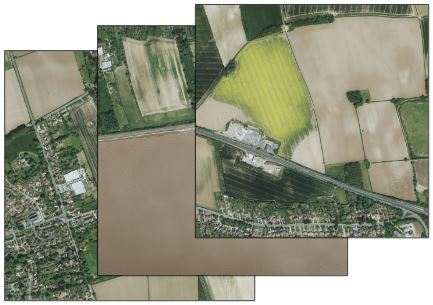
\includegraphics{figs/1/aerial}
    \caption{OS Aerial Images}
    \label{fig:aerial}
\end{figure}

Their flagship product is OS MasterMap, a database that contains information regarding every feature in Great Britain visible from aerial imagery, displayed on a continuous digital map (see figure \ref{fig:mastermap})

\begin{figure}[H]
    \centering
    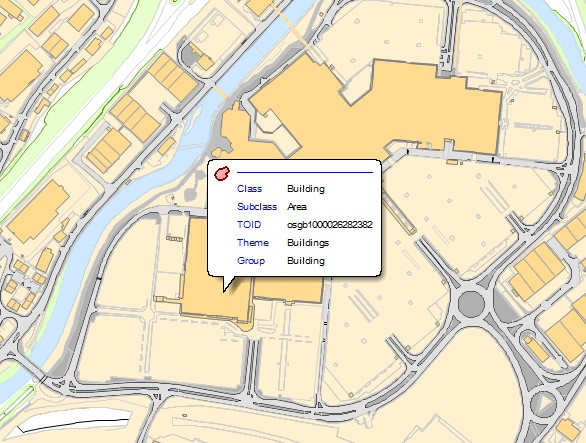
\includegraphics[width=\textwidth]{figs/1/mastermap}
    \caption{OS MasterMap Example}
    \label{fig:mastermap}
\end{figure}

\section{Solution}
OS believe it is possible to automate this process using transfer learning, and have introduced their idea, ``The Productizer'' (see appendix \ref{appendix_proposal}). 
The Productizer will use machine learning to automatically identify features in an aerial image by scanning the image and extracting a hierarchy of attributes from each potential feature. Patterns in these attributes can be used to identify the specific feature, much like a fingerprint. The user will train the tool with supervised data to generate a mapping between the attribute fingerprints and their corresponding feature. 
Using transfer learning, the tool will then scan the rest of the image to find sections that match this fingerprint, thus finding additional occurrences of the feature. The tool would require an easy-to-use interface to hide the complexity of the system, allowing users with no machine-learning experience to train the classifier and obtain its predictions.

\section{Goals}
The goals of the system are as follows:
\subsection{Functional}
\begin{itemize}
    \item Accepts uploading of any Ordnance Survey aerial image
    \item Enables the selection of any feature on the image
    \item Extracts information from selected features that can be used by classification algorithms to identify that feature, much like a fingerprint
    \item Classifier can be trained to identify features using extracted information 
    \item Provides an intuitive interface to easily train the classifier and obtain its predictions, hiding the complexity of the program from the user
    \item Supports iterative training over a dynamic number of classes
    \item Developed as a cloud-based application, usable by multiple users concurrently
\end{itemize}
\subsection{Non-Functional}
\begin{itemize}
    \item Capable of classifying features with an accuracy of 80\%+
    \item Capable of classifying features into 100 separate classes
    \item Processing time for each tile is less than 0.1s
    \item Sufficient supervised training data can be gathered by the user within 5 minutes per class
    \item When used by an expert, results in increased levels of productivity compared to manual identification
\end{itemize}
\subsection{Stretch}
\begin{itemize}
    \item Uses microservices to run separate modules concurrently
    \item Uses contextual information gathered from surrounding tiles to classify tiles
    \item Enables re-training of classifier when it incorrectly classifies a feature
    \item Supports deletion of unfavourable training data
\end{itemize}




\chapter{Existing Systems} \label{chapter:systems}
Mapping is not a very new task: digital mapping gained momentum with the growing popularity for personal navigation devices (like TomTom in 2007, \cite{guardian:tomtom}). However this has all been focused on roads with no consideration to features around the roads. There are however three major organisations who have considered feature and location classification using differing methods:











\section{Google Maps}
Supposedly the market leader in mapping, Google Maps is the most used mapping tool in the world with 1 in 7 people from the entire planet using it at least once a month! Google maps collects it data from a large pool of sources:
\begin{itemize}
 \item \textbf{Map Partners} - Organisations that provide the ``most comprehensive and authoritative data sources" \citep{google:makeusof}
\item \textbf{Satellites} - Until 2014, Google did not own satellites. By investing in satellite businesses, they are provided with images in return \citep{google:satellites}
\item \textbf{Location Services} - By having access to every user's location, users can passively crowd source data.
\item \textbf{Street View} - Ingeniously Google have found many ways of extracting information about features from the images taken on the ground via roaming vehicles.
\end{itemize}.

These are combined in many ways to produce the maps provided on maps.google.com. Google keeps most of these implementations private. However, their engineers often provide hints on the methods used. A technique similar to our own system is the use of satellite imagery for cartography. The image on the left of figure \ref{fig:googlemaps} shows a first layer of processing of a satellite image. 

\begin{figure}[H]
    \centering
    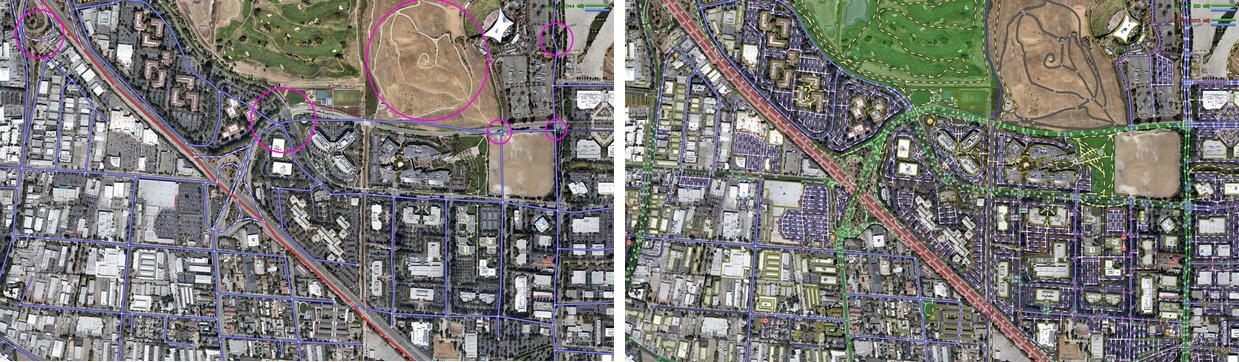
\includegraphics[width=\textwidth]{figs/2/googlemaps}
    \caption{Google Maps Satellite Conversion}
    \label{fig:googlemaps}
\end{figure}

Through the usage of the locations services and manual human editing \citep{google:wired}, the image on the right of figure \ref{fig:googlemaps} is generated. These are then classified by the army of google users. The majority of the work that has been completed was through sheer man-power. Modern techniques are not disclosed to the public. 

A common issue with Google's imagery is that the longitude and latitudes are often incorrect, since the scale in the image is unreliable. The accuracy of labels also reduces the further a tag is from a populated area. Google formally makes no claims on the accuracy of their systems, claiming that their measurements “are provided for entertainment only” \citep{google:forum}.

This leaves Google Maps as a novel system with little industrial usage potential. With methods kept formally hidden and implementation only suggested at through blogs and interviews, Google Maps is not a direct competitor nor useful to design decisions. 







\newpage
\section{Terrapattern} \label{section:existing:terrapattern}
\href{http://www.terrapattern.com/}{Terrapattern} is considered the main competitor in this field. Currently in alpha, it has many of the same features as required by the client. Using the google maps API it has classified every minor tile within the bounds of six cities in the USA and Berlin. It is an open source project available on \href{https://github.com/CreativeInquiry/terrapattern}{github}. 

\begin{figure}[H]
    \centering
    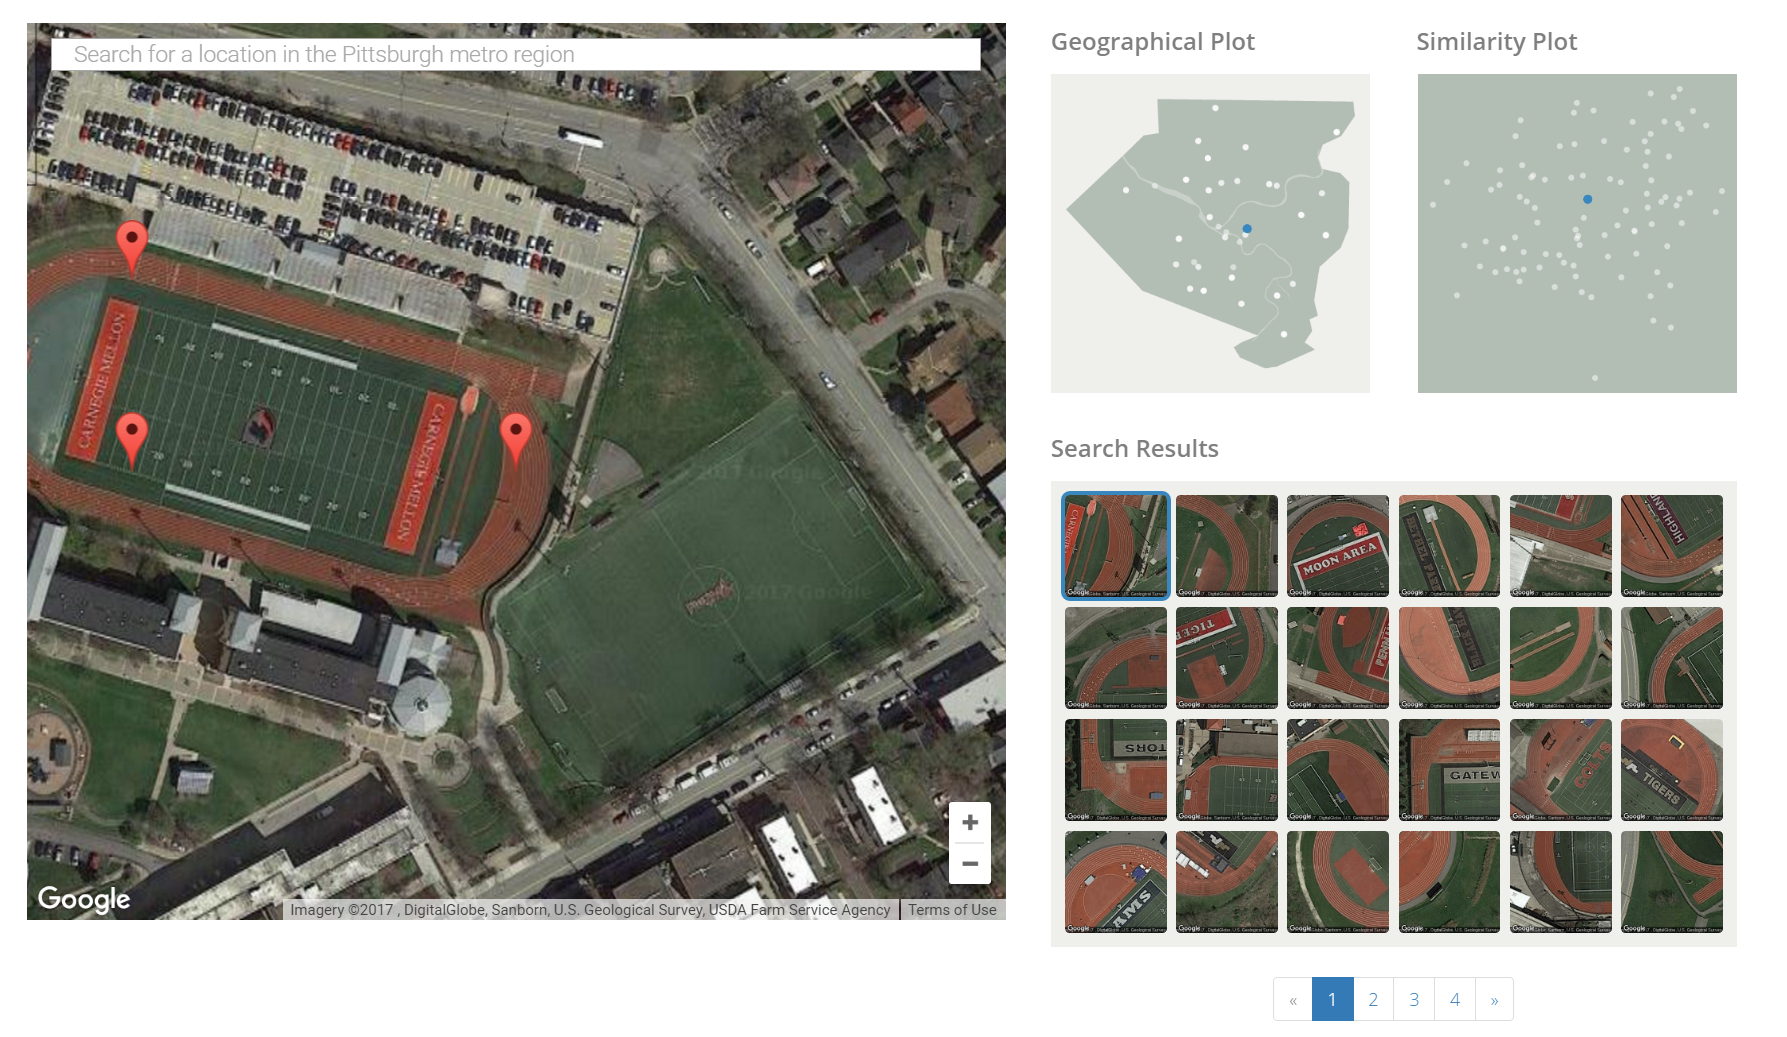
\includegraphics[width=\textwidth]{figs/2/terrapattern}
    \caption{Terrapattern finding corner running tracks in Pittsburgh (USA)}
    \label{fig:terrapattern}
\end{figure}

\subsection*{How it works}
For each city within Terrapattern, an extremely large polygon is selected off of google maps and is tiled. Many labelled features are taken from the OpenStreetMap dataset and processed through a deep neural network (DNN), training it. Then every tile of the city is processed through that DNN in order to classify it \citep{terrapattern:howitworks}.

\subsection*{Pros}
Terrapattern has a very large collection of feature types, with an intriguing precision (e.g. purple tennis courts rather than just tennis courts). Its clear minimaps allow for density of features to be easily observed. Users can search for specific features. This technique is fantastic for identifying and finding similar odd objects, like their example of finding cargo boats or corners of running tracks (figure \ref{fig:terrapattern})

\subsection*{Cons}
The developers of Terrapattern have admitted this is a only a prototype, explaining the reason why it is wrought with flaws. Due to the tiling, it cannot handle the fuzzy border issue that is often accompanied with uniform tiling (The fuzzy border issue is expanded on in section \ref{section:fuzzy}), causing rather unintelligent classifications, as can be seen in figure \ref{fig:bad_terrapattern}. Due to the subtle angle in the streets of San Francisco, identical housing is not identically labelled and roads with trees cannot be continuously discovered. This issue is propagated throughout the map. 


\begin{figure}[H]
    \centering
    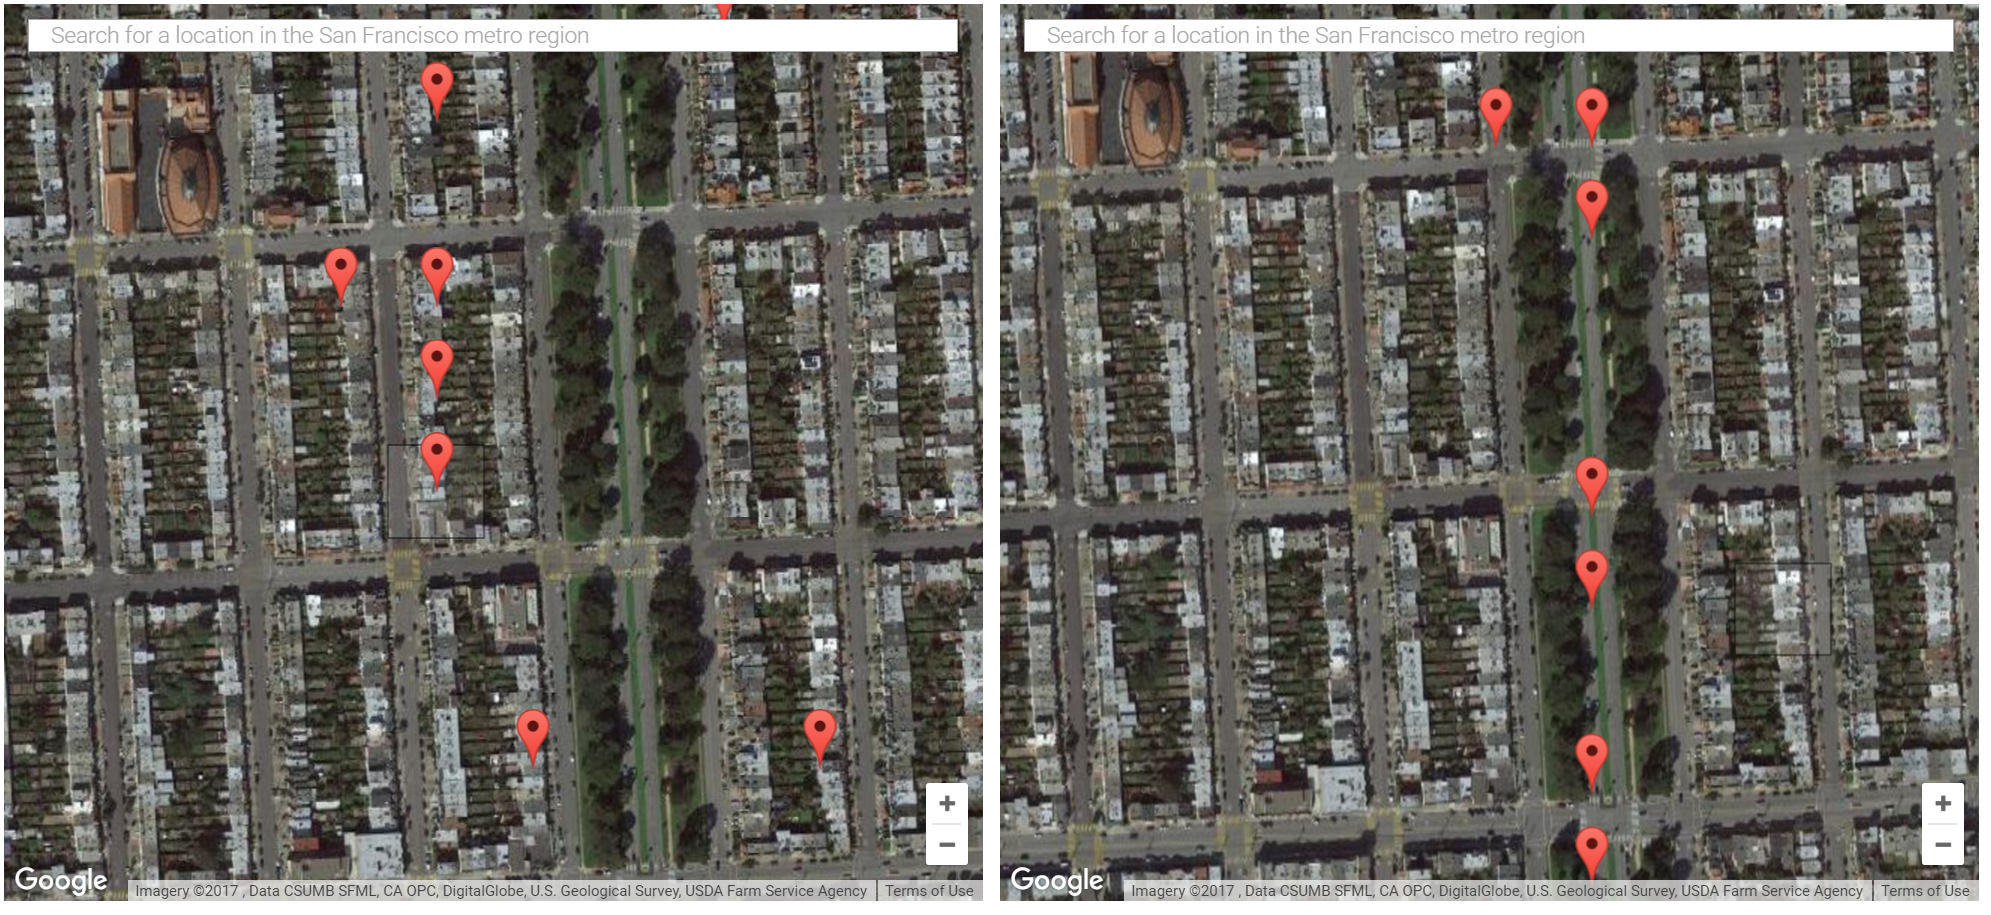
\includegraphics[width=\textwidth]{figs/2/bad_terrapattern}
    \caption{Fuzzy Border Issue in Terrapattern}
    \label{fig:bad_terrapattern}
\end{figure}

The results of Terrapattern are static. They do not allow for any corrections or additions to the map. This prevents the previously mentioned errors from being fixed. This is a serious issue with the semi-unsupervised nature of the model, resulting in the errors remaining there.

The technical components of Terrapattern are evidently strong, however according to their system it is considerably slow. The process of training the DNN took 5 days, and resulted in a top-5 error rate of 25.4\% (\cite{terrapattern:howitworks}), which is unfortunately not that accurate. 

\subsection*{Evaluation}
Terrapattern's approach to the problem is very good. The technical approach and tools themselves are novel. However, the lack of supervised learning and support for supervised learning holds it back. In the context of Ordnance Survey, this makes the method of learning used by Terrapattern near useless as the world is not a series edge cases, but actually full of conformity that this tool cannot easily handle.




\chapter{Planning}
Before any design or work could be done, an appropriate method of organisation had to be chosen:

\section{Waterfall}
Waterfall (and similar) project management styles are linear, stage based development. Each tier of development (as shown in diagram \ref{fig:waterfall}) must be completed before advancing to the next. This approach helps determines issues that could occur later and usually results in better documentation. However, any issue or requirement change requires reverting back to a previous tier \citep{agilevswaterfall}.

\begin{figure}[H]
    \centering
    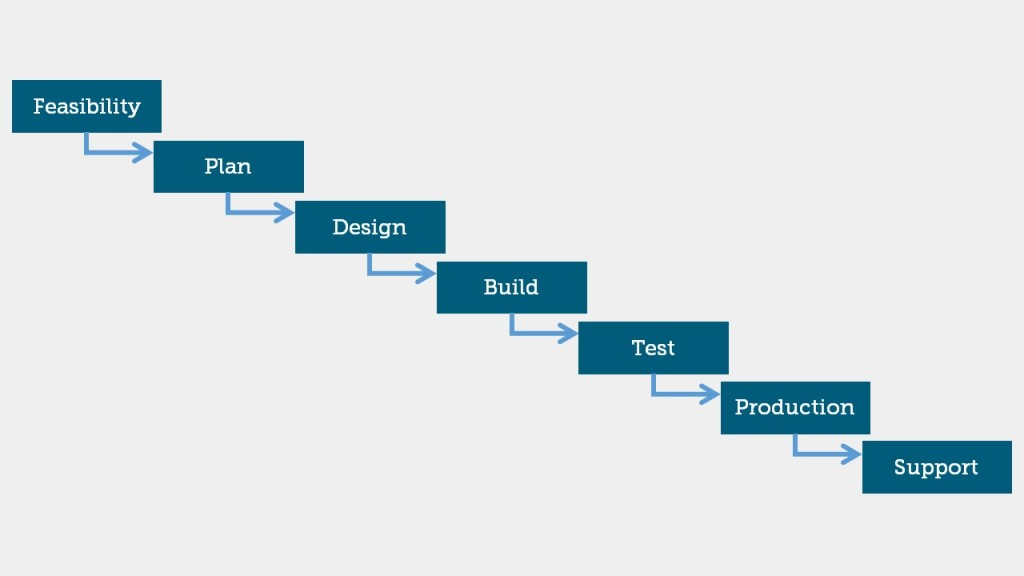
\includegraphics[width=0.8\textwidth]{figs/3/waterfall}
    \caption{Waterfall Stages \citep{agilevswaterfall}}
    \label{fig:waterfall}
\end{figure}

\section{Agile}
Conversely, agile development is a process of continuous, incremental delivery. Each iteration of work is planned briefly and implemented whilst a backlog of work is maintained, allowing for cross functional teams that focus on regular contact with a client leading to short feedback cycles. This ensures that a solution is developed to closer to the customers (often changing) requirements.

\begin{figure}[H]
    \centering
    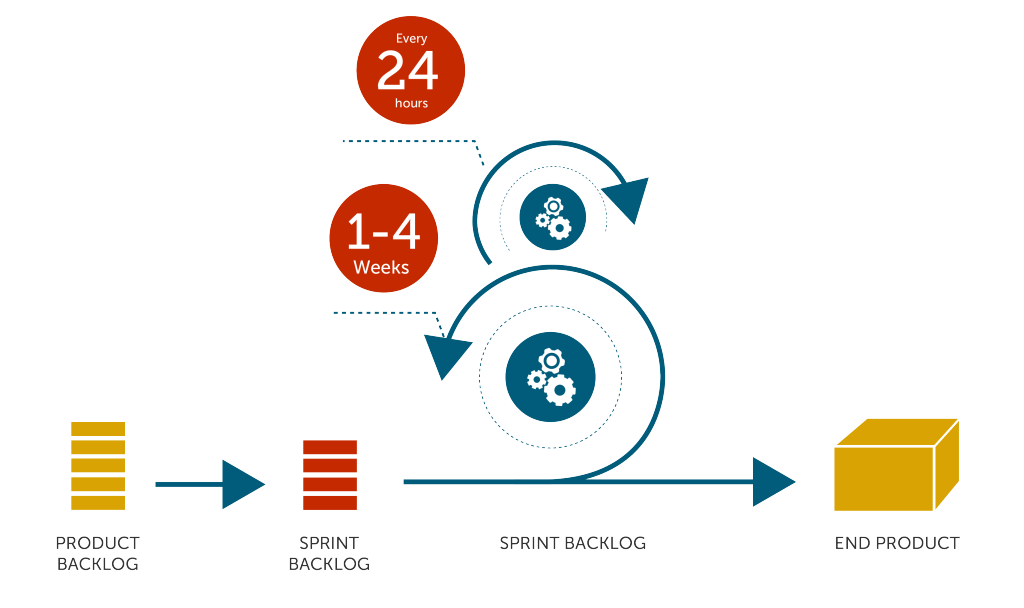
\includegraphics[width=0.8\textwidth]{figs/3/agile}
    \caption{Agile Cycle \citep{agilevswaterfall}}
    \label{fig:agile}
\end{figure}

\section{Outcome: SCRUM}
The agile approach was chosen however agile is an abstract idea. Figure \ref{fig:agile} shows a concrete method of applying the agile methodology to a project. Every iteration (called a `sprint') in scrum lasts one to four weeks and every day the team meet for `stand ups'.


\section{Team Dynamics}
\subsection{Meetings}
As an agile team there would be at least three contact hours a day, every working day. These meetings would be identical to a working day at an agile software development firm. The first hour would often consist of development, followed by a stand up where each team member would update each other on the previous days success and failings and what tasks were to be completed before the next meeting. These `stand-ups' would last no more than 10 minutes. This allowed the team to stay up-to-date with the state of the product. Development would continue afterwards and for 2 hours alone. 

Every week there was a meeting with the project supervisor, where they were updated of the weeks progress and any design changes. These meetings were key to extending our research as the project supervisor had a wealth of knowledge on the subject. Until the third deliverable, the client joined these meetings. This would allow the regular feedback cycles required of SCRUM. Also, by keeping the client up to date, they could steer development. Allowing the project to be built towards the next criteria she desired.

\subsection{Communication}
SCRUM ensured the project was well managed however a key aspect of agile is person to person interaction, not only with the customer but within the team as well (criteria 6 in the agile manifesto \cite{agile:manifesto}). By applying eXtreme Programming (XP) values \citep{XP:values}, this ensured that criteria was fulfilled. 

Respect and communication were key when working in conjunction with SCRUM. A mantra naturally formed ``The work for the team was more important than an individual's''. When a person was stuck on a bug, more team members would help fix it. This close contact also allowed for impromptu design meetings whenever necessary. 

\subsection{Retrospectives}
At the end of each iteration we completed a `retrospective'. This helped us discuss any successes or failures over the previous weeks. It ensured that everyone had a voice and a place to be heard without distraction. This helped us look at the efficiency of our agile process and tailor it to our needs.

In the figure \ref{fig:retro}, you can see the starfish approach was taken. There are five categories, in black, where items are placed that the team should keep doing; do more of; start doing; stop doing and do less of. The team then went through the sections explained what was meant by each point and through this developed actions (as seen in the top left) of tasks that should completed straight after the meeting. The starfish was only one approach to the retrospectives. By doing a different retrospective style or game, it kept what could be a boring meeting into something interesting, creative and most importantly relaxing. 

\begin{figure}[H]
    \centering
    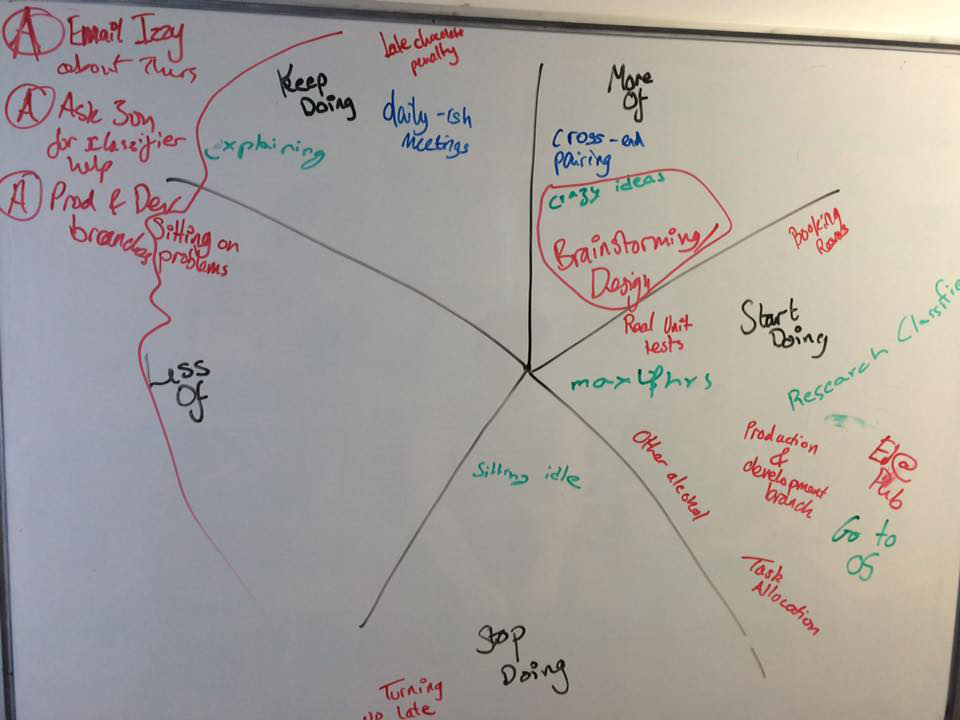
\includegraphics[width=0.8\textwidth]{figs/3/retro}
    \caption{One of our retrospectives}
    \label{fig:retro}
\end{figure}









\section{Project Management}
\subsection{Requirement Elicitation}
In order to create a Gantt chart, it had to determined which tasks were required to complete the project. Therefore in the first week a meeting was held with the project supervisor and industry customer to elicit key requirements from the software and their priorities. Thus emerged the initial task categories:

\begin{itemize}
\item General application
\item Interface
\item Grayscale vectorized images
\item Terrapattern conversion
\item Classifier
\item Feature Finder
\end{itemize}


\newpage
\subsection{MoSCoW}
Then, what these categories consisted of was determined by defining subtasks. In some cases various levels of a function were outlined. For example requirement C1.1 and C1.2 define a differing accuracy available. All of these requirements can be found in `Project Requirements' within appendix \ref{appendix:proj_reqs}. 

They have been prioritized via the MoSCoW method, where each task MUST/ SHOULD/ COULD/ WON'T be completed. This method is excellently intuitive for the customer and allowed for functionality discussions to flow smoothly.


\subsection{Gantt Chart}
Based on the nature of the project, there were two hard deadlines. On the 26$^{th}$ of October and 23$^{rd}$ of November, presentations had to be given on project progress. Therefore it was decided that this provided the team with three 4 week deliverables. Based on the companies we had experience with, 2 week sprints were the ideal balance of workload to work-based pressure.

When scheduling functionality, the ethos was `Minimum viable product'. The main idea being, if the project was dropped the day after a hard deadline, the Productizer would be a fully functioning tool. We also had to take into consideration the workload from other modules would increase over the semester. Therefore we scheduled 50\% of the workload to be complete in iteration one out of three, 30\% in iteration 2 and 20\% in iteration 3. This formed the gantt chart that can be seen in figure \ref{fig:gantt} below. 

\begin{figure}[H]
    \centering
    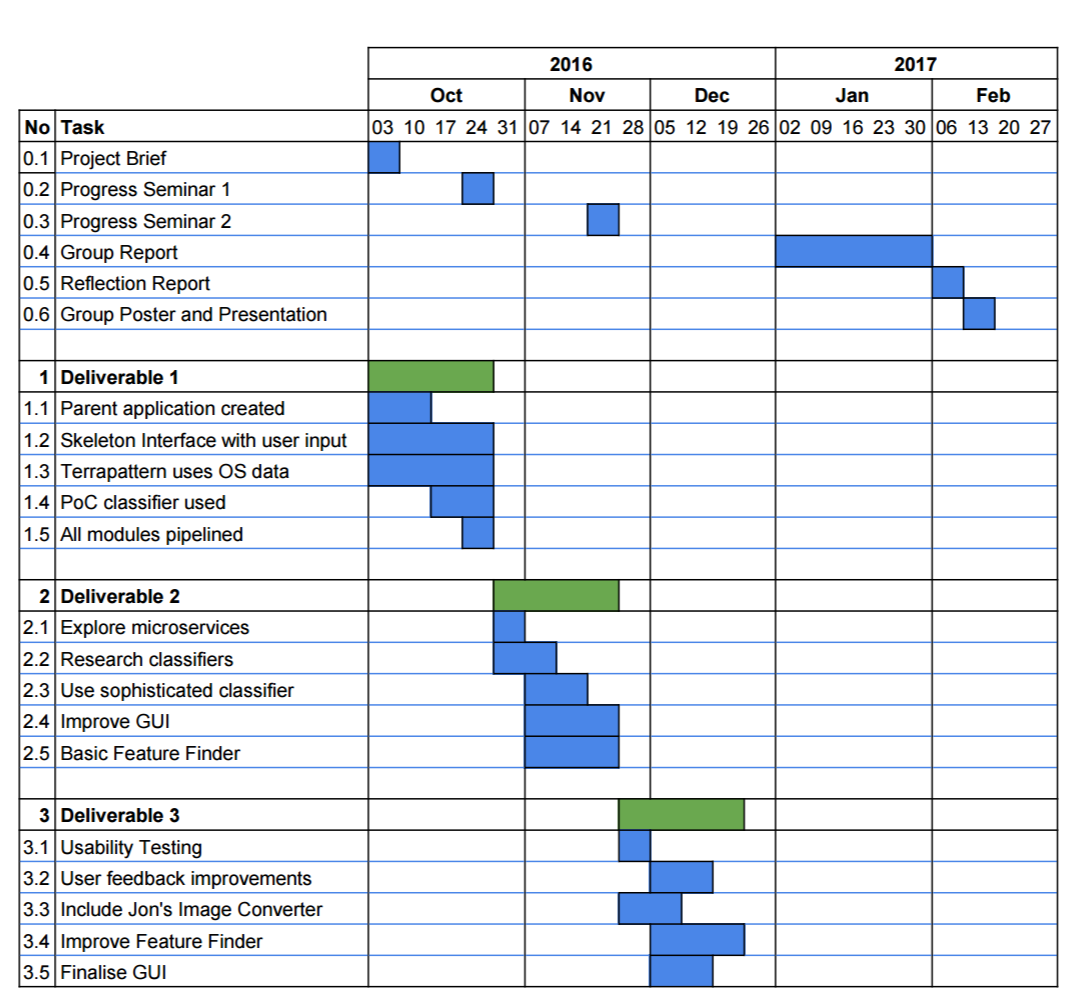
\includegraphics[width=1.1\textwidth]{figs/3/gantt}
    \caption{The Resulting Gantt Chart}
    \label{fig:gantt}
\end{figure}

\newpage

\subsection{Task Allocation}
Each task of a deliverable (from the Gantt chart) is comprised of a number of subtasks. To manage the completion of these tasks and subtasks, we kept sprint boards. 

\begin{figure}
    \centering
    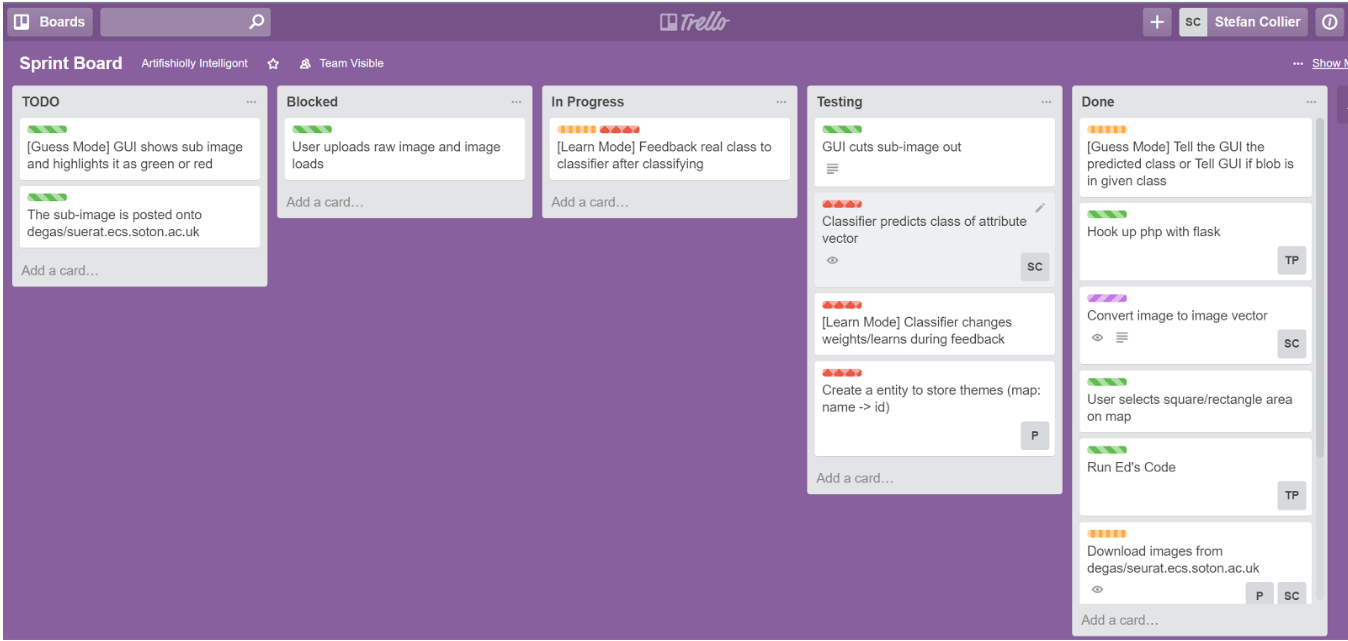
\includegraphics{figs/3/sprint_board}
    \caption{Sprint Board}
    \label{fig:sprint}
\end{figure}

Sprint boards are a fantastic method of scoping where the team is within the sprint. The consist of a number columns defining what stage of development a task is at. Tasks also belong to `Epics' which act as overriding themes (e.g. a GUI Epic). Self organising teams are a key aspect of agile development \citep{agile:manifesto}, as they encourage the best designs. The board enables developers to pick up tasks without concerns of conflict and by using Epics, they can easily guess if they have the domain knowledge for the task. 

\newpage
\subsection{Risk Analysis}
At the start of the project a list was compiled of risks and some contingency plans were completed. Note that impact and probability are out of 5 (where the larger the value implies a larger impact or chance of event). 


\begin{table}[H]
\centering
\label{my-label}
\begin{tabular}{@{}lcccl@{}}
\toprule
Risk                                                                                  & \begin{tabular}[c]{@{}c@{}}Impact\\ I\end{tabular} & \begin{tabular}[c]{@{}c@{}}Probability\\ P\end{tabular} & \begin{tabular}[c]{@{}c@{}}Rating\\ (P * I)\end{tabular} & Contingency                                                                                                         \\ \midrule
Ed going on holiday                                                                   & 4                                                  & 5                                                       & 20                                                       & \begin{tabular}[c]{@{}l@{}}- Deliverable-worth of work before \\ going\\ - Ed does handover\end{tabular}            \\ \midrule
\begin{tabular}[c]{@{}l@{}}Coursework from \\ other modules\end{tabular}              & 3                                                  & 5                                                       & 15                                                       & \begin{tabular}[c]{@{}l@{}}- Iteration 1 contained majority of\\  tickets(before courseworks released)\end{tabular} \\ \midrule
\begin{tabular}[c]{@{}l@{}}Team member\\  disappears/ is ill\end{tabular}             & 5                                                  & 1                                                       & 5                                                        & \begin{tabular}[c]{@{}l@{}}- Ensure no single specialists\\ - Share knowledge\end{tabular}                          \\ \midrule
\begin{tabular}[c]{@{}l@{}}Difficulty working \\ with Terrapattern\end{tabular}       & 3                                                  & 3                                                       & 9                                                        & \begin{tabular}[c]{@{}l@{}}- Use alternative image attribute\\  extractor\end{tabular}                              \\ \midrule
\begin{tabular}[c]{@{}l@{}}University source control \\ becomes unstable\end{tabular} & 5                                                  & 3                                                       & 15                                                       & - Use professional source control                                                                                   \\ \bottomrule
\end{tabular}
\caption{Key Considered Risk}

\end{table}

\section{Code}
\subsection{Pair Programming}
Pair Programing is the process of development where two people work together on one workstation to write code. By constantly swapping, both parties remain engaged \citep{pairing}. The main way to pair is the `Driver and Navigator' scenario. This is when two decide on a functionality to add and then the `Navigator' informs the `Driver' of instructions to perform; whilst checking the code for any bugs. 

During the first iteration, pair programming was used heavily. Due to the team's inexperience with the Python language this helped produce reliable code. When the experience party played the navigator, the driver learnt as they typed. When both parties were inexperienced then it helped prevent the driver from getting stuck as the navigator can determine what knowledge might be needed as the driver was writing. As the team became more experienced with Python, pairing occurred less frequently; being used for major or complex functions. 

This technique significantly reduced the need for peer reviewing work. It also ensured a transfer of knowledge in two ways. Participants learnt the language together, learning together was much faster than alone. This resulted in code quality increasing at a much faster rate and technical debt reducing each week. Participants also learn how other sections of the code functioned. This stopped the `reinvention of the wheel', auxiliary tools and helper functions were well known and widely used where necessary. 

\subsection{Distribution of Knowledge}
The team meetings (or `work days') of the first week of iteration 2, were strictly reserved for machine learning training. This was essential as only one team member had machine learning (ML) knowledge, research and development of ML-based systems was too much work for one person. The ML experience member taught the two server-side members the basics of machine learning, supervised, unsupervised learning techniques and briefly explained semi-supervised learning. 

This knowledge allowed the the entire server side team complete a group spike to determine the best classifier for the system. Not to mention being able to understand the code and intended purpose of it, which greatly helped testing. 


\subsection{Peer Review}
At the end of any significant task (that was completed individually), a developer would run through their work with another team member. Allowing for a the distribution of knowledge and bug checking that would have occurred if they pair programmed. This made certain of a good standard of code and reduced code redundancy whilst allowing both developers to make progress on separate tasks.

\subsection{Git}
In order to manage code version control, git and Github were used. All code was hosted as an `organisation' on github where our code could be privately managed. Each microservice had its own code repository to ensure modularity, thus avoiding merge issues during synchronous work. 

When doing day to development, code would be merged to the `dev' branch. The virtual machines would run off of the `prod' (i.e. production) branch. `dev' would be merged to `prod' once a fully tested and functioning feature had been completed. Therefore the services hosted on the virtual machines could be trusted during singular node testing. 






\section{Dev Tools and Tech}
In order to facilitate pair programming all server side code was written in the same IDE and likewise with the client side. Server side development was all handled via Pycharm and client-facing code was developed using Sublime Text 3. Uniformity was key amongst virtual machines as well, they all ran on Ubuntu 16, loaded with the same .bashrc and apache \& wgsi settings. However development occurred on both OSX, Ubuntu and Windows 10, all with varying screen dimensions. This allowed for various configurations to be tested for the client application.


\section{Division of Responsibilities}
The team consisted of 4 members. Each member had varied expertise and experience with concepts and tools. The team was collectively responsible for each all the code however table \ref{table:focus} shows how the team members distributed their time regarding the two sides of the project:

% Please add the following required packages to your document preamble:
% \usepackage{booktabs}
\begin{table}[H]
\centering
\caption{My caption}
\label{table:focus}
\begin{tabular}{@{}ll@{}}
\toprule
Team Member & Focus                                   \\ \midrule
Edward      & Client Facing                           \\
Prem        & Server Side                             \\
Stefan      & Server Side                             \\
Thomas      & Client Facing (33\%) \& Server Side (66\%) \\ \bottomrule
\end{tabular}
\end{table}

Even though each member shared the work of each service, by having a guardian for each service ensured there were final checks and tests. It also ensured that each team member had a particular expertise that helped when problems or questions were directed to the team: 

% Please add the following required packages to your document preamble:
% \usepackage{booktabs}
\begin{table}[H]
\centering
\begin{tabular}{@{}ll@{}}
\toprule
Team Member & Main Service          \\ \midrule
Edward      & Productizer (\&Grunt) \\
Prem        & Saturn                \\
Stefan      & Olivia                \\
Thomas      & Classifier            \\ \bottomrule
\end{tabular}
\caption{Key Responsibilities}
\end{table}




\chapter{Technical Approach}\label{chapter:tech}
\section{System Overview}
Figure \ref{fig:sys_overview} provides a high-level overview of the system architecture. The system consists of several microservices, each of which perform a unique function. 

The client facing side, the ‘front-end’, of the application, displayed in yellow (see \ref{fig:sys_overview}), consists of Productizer and Grunt. The Productizer provides a graphical interface through which the user can interact with the system, providing training data from uploaded images to the back-end of the system, and adding images that require classification in batches to the Amazon Simple Queue Service (SQS) queue. The queue worker, Grunt, takes images from the SQS queue and sends them to the back-end for processing, writing their classifications to the front-end database, and publishing notifications to PubNub when a task has been processed.

The server side, or ‘back-end’ of the application, displayed in blue (see \ref{fig:sys_overview}), consists of Saturn, Olivia and the Classifier. Saturn acts as the central point of communication, forwarding requests to Grunt, Olivia and the Classifier. Olivia is responsible for downloading images and extracting a 1024-attribute vector from them. The Classifier uses these vectors to predict the class of the image.

\begin{figure}[H]
    \centering
    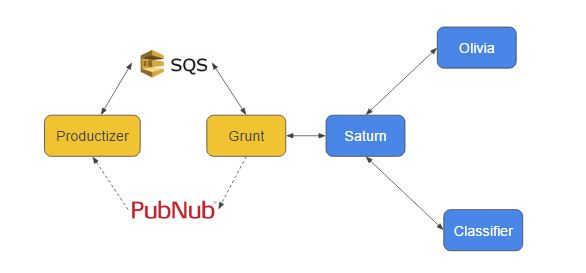
\includegraphics[width=\textwidth]{figs/4/sys_overview}
    \caption{High-level overview of the system architecture}
    \label{fig:sys_overview}
\end{figure}

\section{Requirements}
Before beginning development, requirements were gathered based on the requests of the customer and the needs of the system, details of which are outlined below.
\subsection{Functional Requirements} \label{funcreqs}
\subsubsection{Image Uploading}
The user will be able to upload any Ordnance Survey aerial image. These images could be of any size, and across a range of qualities.
\subsubsection{Feature Selection}
The user will be able to select any feature visible on the image. Despite using tiling, the user will be able to select features that sit on the borders of two tiles. 
\subsubsection{Attribute Extraction}
The system will extract information from selected features, allowing them to be identified.
\subsubsection{Feature Identification}
The system will use classification algorithms, trained with supervised training data gathered by the user, to identify features based on the extracted information.
\subsubsection{Iterative Training}
The user will be able to iteratively train the system over time by providing additional training data for existing classes and new ones. 
\subsubsection{Intuitive Interface}
The system will have an intuitive interface that will be used to train the classifier and obtain its predictions, while hiding the complexity of the program from the user, such that no knowledge or experience with classification algorithms is required.

\subsection{Non-Functional Requirements} \label{nonfuncreqs}
\subsubsection{Accuracy}
After sufficient training, the system will be capable of classifying features with an overall accuracy of 80% or more.
\subsubsection{Scalability}
The system will be capable of identifying 100 unique features without significant reduction in performance.
\subsubsection{Speed}
The system will process each 256x256 tile of an image in under 0.1s.
\subsubsection{Usability}
Using the user interface, the user will be able to provide the system with sufficient training data to identify a new class under 5 minutes.
\subsubsection{Productivity}
Over a substantial period of time, an experienced user of the system will have higher levels of productivity (i.e a faster rate of feature identification) compared to that same user identifying features manually.

\subsection{Implementation Requirements} \label{impreqs}
\subsubsection{Language}
\subsubsubsection{Front-end} \label{frontendlang}
The front-end application must allow for communication with a MySQL database, as well as provide the ability to serve a HTML/CSS based website. The application must be able to run front-end JavaScript in order to provide support for Google Maps API, allowing image manipulation. Furthermore, the application should allow the uploading and retrieval of images that can be used within the map display. 
\subsubsubsection{Back-end} 
The back-end language must allow for fast development, with access to relevant third-party module, such as classification algorithms and HTTP communication libraries. Additionally, it should be compatible with Olivia’s attribute extraction code, which was written in Python.
\subsubsection{Persistence}
\paragraph{Front-end\\}
Persistence is used in the front-end to:
\begin{itemize}
    \item Store initial uploaded image, and all tiles generated from this
    \item Store maps in database with unique ID, link to image path, and further details
    \item Store tiles in database, associated with specific map, along with their coordinates and classifications
\end{itemize}
\paragraph{Back-end\\}
Persistence is used in the back-end to:
\begin{itemize}
    \item Map image IDs to extracted attributes in the Attribute Extractor
    \item Store all training data in the classifier microservice
    \item Map Feature ID Number to Feature Name in the classifier
\end{itemize}
\subsubsection{Front-end}
The front-end of the application must be accessible by multiple users concurrently from any location. 
\subsubsection{Platform}
The back-end of application must run on a platform that makes it available to a wide audience.
\subsubsection{Framework}
The framework must be quick to learn due to the limited time available. Only basic utility is required from the framework for the purposes of this project. The two main options available in Python are Flask and Django. 
\subsection{Interface Requirements} \label{intreqs}
\subsubsection{Image Manipulation}
The interface will allow the user to upload any Ordnance Survey aerial image, pan around the image and select any visible feature on the image. It should also provide quick access to previously uploaded images. 
\subsubsection{Interaction with Classifier}
The interface will allow the user to interact with classifier, providing supervised training data for existing and new classes, and obtaining the its predictions. The interface will be simple and easy to use, hiding the complexity of the classification algorithm, such that no experience in machine learning is required.
\subsection{Use Case Analysis}
Figure \ref{fig:comic} was produced during the initial use case analysis of the project, providing a high-level overview of the functionality required by the system.
\begin{figure}[H]
    \centering
    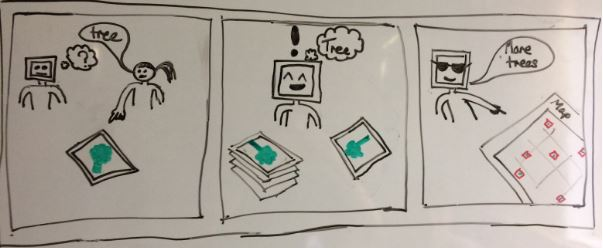
\includegraphics[width=\textwidth]{figs/4/comic}
    \caption{A comic strip produced to provide a high-level overview of system functionality}
    \label{fig:comic}
\end{figure}

Following this comic strip, a formal use case diagram was produced, as shown in figure \ref{fig:use_case_diagram}. As shown in the diagram, users will be able to upload their own map or work on previous maps. They can then select Learn Mode and train the classifier by selecting features and providing their true class, or select Discover Mode and obtain the classifier’s predictions, filtering the output to show the feature they are looking for. They can create new classes, and after providing sufficient training data, reclassify the map to find occurrences of this new feature.  
\begin{figure}[H]
    \centering
    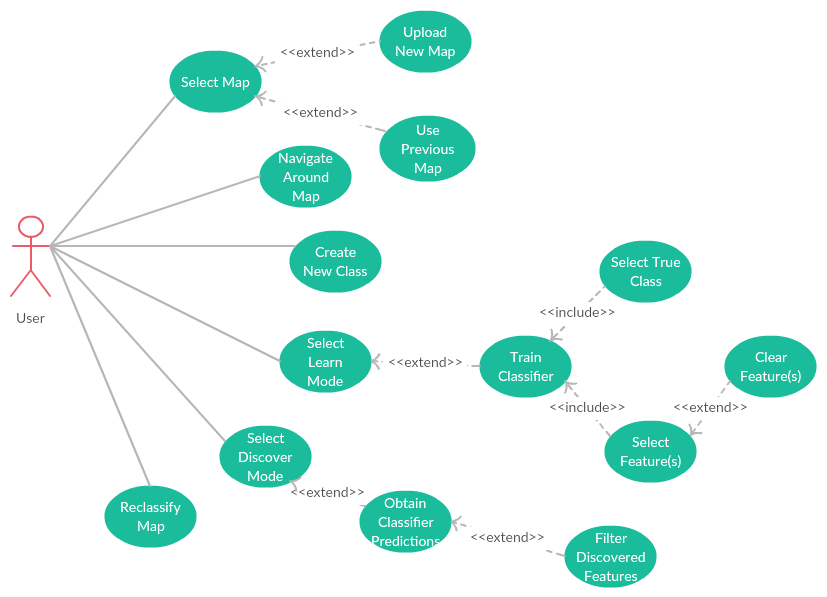
\includegraphics[width=\textwidth]{figs/4/use_case_diagram}
    \caption{The System Use Case Diagram}
    \label{fig:use_case_diagram}
\end{figure}

\section{Design}
\subsection{Overview}
Having considered the system requirements, a number of design choices were made to ensure the system met these requirements. 
\subsection{Design Choices}
\subsubsection{Language}
\paragraph{Front-end\\}
PHP was used to ensure all of these requirements outlined in \ref{frontendlang} are met. Additionally, PHP provides a vast community of developer support and a number of pre-built frameworks that can enhance speed of development.
\paragraph{Back-end\\}
Python was chosen as the back-end development language due to the fast code development and vast quantity of third-party support offered. Additionally, using Python ensures compatibility with Olivia’s attribute extraction code, allowing for flexibility in the system architecture. 
\subsubsection{Persistence}
\paragraph{Front-end\\}
All images are stored in the application file system to maintain front-end persistence. In order to store the map and tile details, a MySQL database was used in order to create a relational database that could link the tiles with their associated map. PHP provides secure functions to interact with MySQL databases to negate the risk of SQL injection, plus frameworks such as Laravel provide Object-relational mapping to allow abstraction from direct SQL queries.
\paragraph{Back-end\\}
CSV files were used for the back-end persistence, since a simple storage system with read-all and write-all functions is all that was required. Python supports this method of storage with a CSV module, providing all required functions. Additionally, this approach is lightweight and easily implemented. 
\subsubsection{Front-end}
A cloud-hosted web application was used for the user interface of the application, allowing it to be accessed by multiple users concurrently.
\subsubsection{Platform}
The back-end of the application was designed to ensure it could be run on Linux. 
\subsubsection{Framework}
Flask was selected over Django as the framework for the project. While Django is more powerful, this comes at the price of a steeper learning curve, whereas Flask supports all of this project’s requirements and also can be learnt relatively quickly.
\subsection{Iterations}
\subsubsection{Iteration 1}
\paragraph{Overview\\}
While using an agile methodology, it is important to ensure that a minimum viable product is developed by the end of each iteration. Based on this concept, the following simple client-server architecture was implemented during the first iteration (Figure \ref{fig:iteration1_overview}). 
\begin{figure}[H]
    \centering
    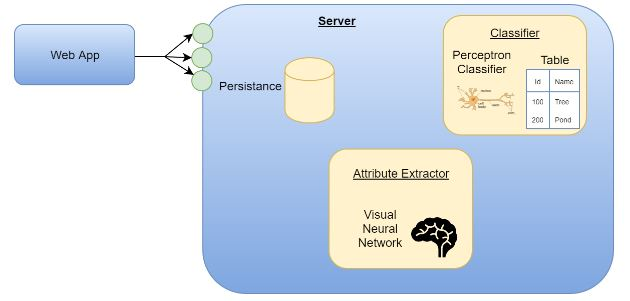
\includegraphics[width=\textwidth]{figs/4/iteration1_overview}
    \caption{An overview of the client-server architecture implemented in Iteration 1}
    \label{fig:iteration1_overview}
\end{figure}
\paragraph{Client Side\\}
On the client side, a fully-functional GUI was developed, allowing the user to upload any map, access previously uploaded maps, and zoom and pan around the map. Tiling was used, splitting the map into 256x256 pixel tiles, allowing the user to select features by clicking its nearest tile.
\paragraph{Server Side\\}
On the server side, image attribute extraction was performed using code from previous student Olivia Wilson’s Masters project. This code was run on the CPU, providing a slow but functional extraction of 1024 attributes from each 256x256 tile.

To perform this extraction, the image must first be downloaded onto the server. Therefore, memory persistence was used to store images until they have been processed.

Additionally, a Perceptron was implemented as a proof-of-concept classifier. This used the extracted attributes either for supervised training or to provide basic predictions. It made use of a table to convert human-readable feature names to perceptron-useable ID numbers. 
\paragraph{Functionality\\}
These components were used to develop a product capable of two modes: Learn Mode and Guess Mode.

In Learn Mode, the user would upload an image, select a number of tiles containing features, provide the name of the feature, and click ``learn”. A HTTP POST request containing the URLs of the selected tiles was sent to the server. The server downloaded the images from the given URLs and extract their attributes into a vector. Additionally, the feature name was converted to an ID number using the lookup table. Finally, the perceptron was trained using the vectors and class ID number via supervised learning.

In Guess Mode, the user would upload an image, select a single tile, and click ``guess”. Again, on the server side the image was downloaded and its attributes extracted. The perceptron then guessed the class ID of the tile based on its attribute vector, converted this ID to a string using the lookup table, and returned the guess. The web application then displayed the predicted class to the user.

\subsubsection{Iteration 2}
\paragraph{Overview\\}
After developing a broad yet shallow product in iteration 1, the focus of iteration 2 was to add depth to the system. The client-server architecture was improved through the addition of microservices, as shown below (Figure \ref{fig:iteration2_overview}).
\begin{figure}[H]
    \centering
    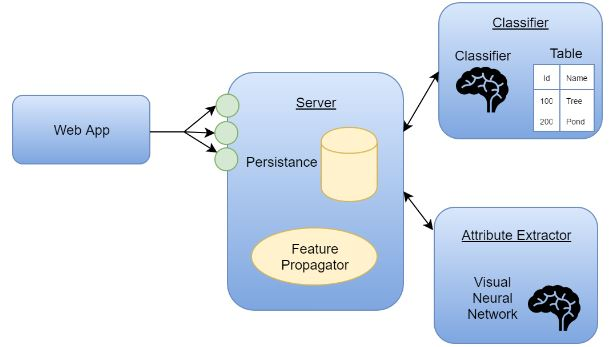
\includegraphics[width=\textwidth]{figs/4/iteration2_overview}
    \caption{An overview of the microservices architecture implemented in iteration 2}
    \label{fig:iteration2_overview}
\end{figure}
\paragraph{Web Application\\}
The web application was improved through the inclusion of Amazon SQS and PubNub. The web app now adds each image-to-be-processed to the SQS queue. The queue worker, Grunt, retrieves images from this queue and forwards them to the back-end. After an image has been processed and classified, Grunt publishes the image along with its classification results to PubNub. The web app displays PubNub classifications on the map, allowing the user to identify features of a selected class. Additionally a completion bar was displayed, showing the progress of image processing based on entries remaining in the SQS queue.
\paragraph{Server\\}
The functionality of the server was moved into separate microservices, and its responsibility was now to act as the central point of communication between microservices. Additionally, it contained global data persistence for the classifier and attribute extractor, as well performing the logic used for feature finder (discussed in \ref{ittwo-classifier}) by filtering out irrelevant classes. 
\paragraph{Attribute Extractor\\}
The attribute extractor was now running as an independent microservice, hosted on a powerful machine with a GTX Titan X GPU, containing 3072 cuda cores and 12GB ram. To take advantage of this, the code was modified to run on the GPU rather than CPU. Running on the CPU, the code would take approximately 30 seconds to process a single 256x256 image, whereas on the GPU it could process a batch of 128 images concurrently in 0.1 seconds, reducing processing time by a scale of 38,400. 
\paragraph{Classifier\\} \label{ittwo-classifier}
Also now running as an independent microservice, the classifier saw a number of improvements. The perceptron algorithm used was replaced with a Support Vector Machine. This algorithm provides significantly more accurate predictions with much less training data required (see section 8 for a full list of advantages and limitations). Additionally, knowledge persistence was implemented in the classifier, storing all supervised training data it uses. This allows the classifier to learn iteratively by incrementally adding data to the storage, as well as enabling its knowledge to be easily controlled, since sub-optimal training data can be deleted and forgotten.
\paragraph{Functionality\\}
The changes listed above resulted in a number of non-functional improvements to the system: greater concurrency reducing overall processing time, faster image processing, greater prediction accuracy. Additionally, the functionality of the system was improved. 

The proof-of-concept Guess Mode implemented in iteration 1 was extended into Discover Mode in iteration 2. Rather than guessing the class of a single tile selected by the user, Discover Mode gathers the predicted class of all tiles in an image. The user can then select the feature they wish to discover, and all identified occurrences of that feature are highlighted on the map. 

\subsubsection{Final Iteration}
\paragraph{Overview\\}
By the end of iteration 2, the developed system met the specification outlined at the start of the project. The final iteration was used predominantly for bug fixes, usability testing, improvements and extensions. 
An overview of the final architecture of the system can be seen below (figure \ref{fig:iteration3_overview}).
\begin{figure}[H]
    \centering
    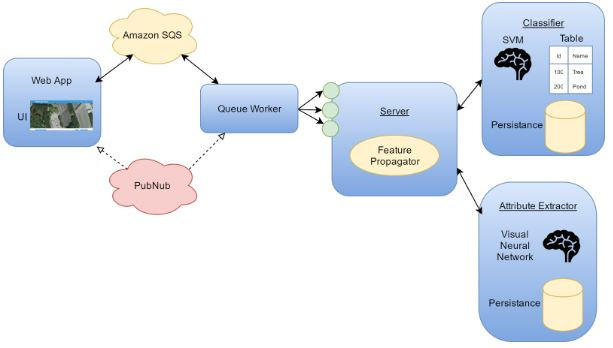
\includegraphics[width=\textwidth]{figs/4/iteration3_overview}
    \caption{An overview of the finalised architecture of the system}
    \label{fig:iteration3_overview}
\end{figure}

\paragraph{Web Application\\}
Following the feedback from usability testing, a number of improvements were made to the web application.

A highlighting square was added to the map display, outlining the boundary of the selected tile. This was used in Learn Mode to help the user to select the correct tile, and Discover mode to provide context to feature markers by showing the tile they correspond to. 

Additionally, by using 256x256 tiles, occasionally a feature would sit on the boundary between two tiles, making it unselectable. Therefore, the tiling system was revised to instead combine four adjacent 128x128 tiles to generate the 256x256 tile. This resulted in overlapping 256x256 tiles, allowing previously unselectable features to be selected. 

Finally, discover mode was improved by using a checkbox for the classes to be discovered, allowing multiple classes to be selected and discovered at once. To visualise this clearly, a different coloured marker was used for each class.  

\paragraph{Attribute Extractor\\}
Previously, the attribute extractor would download every tile image before extracting its attributes, and would often need to process the same tile multiple times. However, downloading images is the most significant bottleneck in system performance, and the extracted attributes never change for the same image.

Therefore, each tile was assigned an ID number based on its map ID, X coordinate and Y coordinate. After downloading a tile image and extracting its attributes, this vector is stored in a table, with the ID number as the key. Whenever a tile requires processing, the attribute extractor first checks for its ID number in the table, returning the corresponding attribute vector if it exists. This ensures each tile is only downloaded and extracted at most once. 

Additionally, a problem with Olivia’s attribute extraction code is that, given a 256x256 image, it only classifies the central pixel, using the surrounding 192x192 pixels as context, and ignoring the outer 32 pixel border. To solve this, the focus of the classification was shifted to 9 positions around the centre of the image, allowing for full coverage. Classification was obtained at each position, allowing probabilities to be calculated based on the distribution of predictions. 
\paragraph{Functionality\\}
As all the functional requirements system were achieved by the end of iteration 2, this final iteration was focused on achieving the non-functional requirements of the system, hence no additional functionality was added.

\subsubsection{Interaction Diagram}
The Interaction Diagram below (figure \ref{fig:interaction_diagram}) shows the interactions between microservices when the user uploads a new map.

The web application splits the image into a number of 256x256 tiles. The URLs of these tiles are sent to Saturn, which forwards them to Olivia to obtain the vector of 1024 attributes. Saturn then forwards the attributes to the Classifier, which returns a predicted class for each tile. These predictions are returned to the web application, where they are displayed on the map to the user. 
\begin{figure}[H]
    \centering
    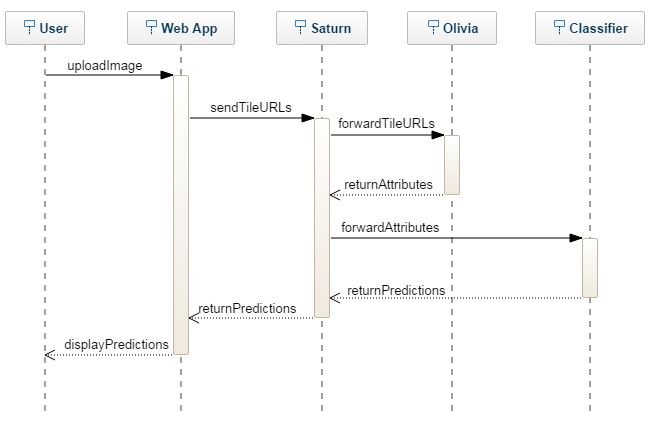
\includegraphics[width=\textwidth]{figs/4/interaction_diagram}
    \caption{An Interaction Diagram showing the process that occurs when the user uploads a map image}
    \label{fig:interaction_diagram}
\end{figure}

\subsubsection{Entity Relationship Diagram}
The following entity relationship (ER) diagrams show the entities that exist within each microservices of the system, the attributes of these entities, and the relationships between them.
\paragraph{Web Application\\}
Figure \ref{fig:webapp_er} shows the entities present in the web application. Starting with a map, a number of tiles are generated, and identified from the map ID, and the X and Y coordinates of the tile on the map. 
\begin{figure}[H]
    \centering
    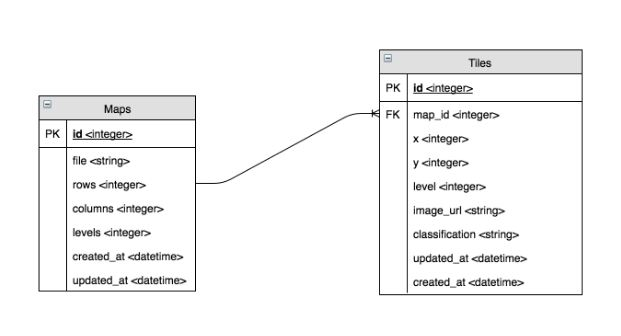
\includegraphics[width=\textwidth]{figs/4/webapp_er}
    \caption{Web Application Entity Relationship Diagram}
    \label{fig:webapp_er}
\end{figure}
\paragraph{Attribute Extractor\\}
In the Attribute Extractor microservice, each of the tiles provided by the web application are processed to obtain information that can be used by the classifier. Before processing a tile, it must first be downloaded from the given image URL to a specific file location. The tile is then processed to obtain a large array of doubles representing the attributes of the tile, which can be used by the classifier.
\begin{figure}[H]
    \centering
    \includegraphics[width=\textwidth]{figs/4/olivia_er}
    \caption{Attribute Extractor Entity Relationship Diagram}
    \label{fig:olivia_er}
\end{figure}
\paragraph{Classifier\\}
In the Classifier microservice, each of the tiles provided by the web application are classified using the information provided by the Attribute Extractor. Upon receiving an image and its corresponding attribute vector, the classification algorithm determines the predicted class of the tile. The class is represented primarily using an ID number, but a human-readable string is used to represent the name of the feature. 
\begin{figure}[H]
    \centering
    \includegraphics[width=\textwidth]{figs/4/classifier_er}
    \caption{Classifier Entity Relationship Diagram
}
    \label{fig:classifier_er}
\end{figure}
\subsubsection{Endpoint Reference Contracts}
An Endpoint Reference Contract provides detailed information for a list of endpoints required by the system. Figure \ref{fig:classifier_endpoints} below provides an example of an endpoint reference contract used by the Classifier microservice. A full list of the endpoint reference contracts used throughout the system can be found in the appendix. Working to these contracts ensures autonomy and seamless integration between front-end and back-end. 
\begin{figure}[H]
    \centering
    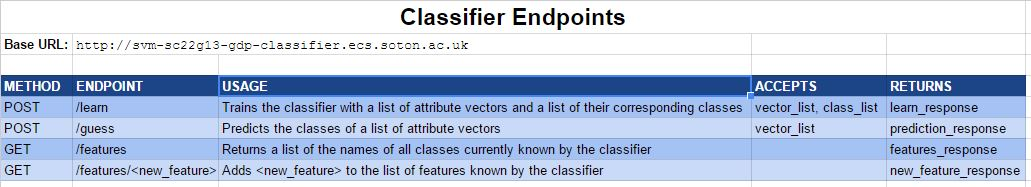
\includegraphics[width=\textwidth]{figs/4/classifier_endpoints}
    \caption{ Endpoint Reference Contract extract for the Classifier}
    \label{fig:classifier_endpoints}
\end{figure}

\chapter{Micro Services Architecture} \label{chapter:MSA}
\section{Overview}
The Micro Services Architecture (MSA) is an efficient way of designing an application where suites of small services, each running its own process, communicate with each other to run a single application. Each of the services are loosely coupled and designed to work as cohesive components of a system.
Our implementation of this architecture comes with design choices for better performance of the system. Performance is discussed in the latter in this part of report. This chapter also discusses some of the disadvantages that can be observed in a micro-services architecture.
\section{Background Research}
The internet contains numerous web-applications and services that are severely limited by their interoperability. Their design promotes access to web-content rather than web services.. In an ideal world, everything should be comprised of web services, whom are all semantically labelled. This would enable an autonomous agent to discover, invoke, compose and monitor resources provided by a service. Everything on the web should be semantically clear to an automated agent so that it is able to discover, invoke, compose and monitor Web resources offering particular services and their properties \citep{martin-2004}. There is extensive research into making the Internet a more versatile platform, where applications are independent, composed and semantically meaningful. Making it possible for automated agent to execute them \citep{MSA}. Web-service architectures such as RESTful, OWL-S, WSMO, etc are some of the approaches that attempt to describe services and process the respective description enabling task automation such as execution. They often form key nodes in MSA systems. 

The Micro-services architecture is a framework to simplify the process of giving semantic meaning to the web service. Each service has a set of descriptive terms which represent a feature. For example, a feature can be a service that performs some kind of user authentication. Breaking a single application into multiple small services which focuses on performing one thing well, helps to bring that independency which is easier to provide semantic meaning to it. Not only the services are reachable from outside, it has also contributed in making a versatile system whose components can be easily replaced or upgraded without altering the whole system.

Whenever a new service is deployed, it must be described to make it available to automated agent. That requires describing its input and output semantically which details operation service performs. It is a time-consuming process and sometime ignored, however can provide great benefits. 
\section{Design}
\subsection{Design Decision}
\subsubsection{Micro-Services Architecture (MSA) vs Monolith Architecture (MA)}
Micro-Services and Monolith architecture are two different software development techniques adapted in many application building processes. MA applications are built as a single unit whereas MSA applications are composed of multiple smaller services which work together as a single unit.
Monolith architecture limits re-usability and can be confusing to group of developers to understand the core objective due to its enormity. It's not agile as it retracts from the takes away the flexibility of code when coding \citep{mulesoft_2016}.
On the other hand, MSA promotes Unix philosophy i.e. ``Do one thing and do it well''. Each service is independent, automated and self-composed which provides resiliency, agility and efficiency. Application can perform better, experience less downtime and can scale on demand \citep{mulesoft_2016}, Due to the context of making a prototype for OS and the flexibility and semantic implications of the approach, MSA is the obvious choice.
\subsubsection{HTTP 200 Error Status}
An emerging practice is returning the HTTP 200 OK status code with a Boolean `success' variable to indicate success or failure of a services request. It provides a simplicity and uniformity when dealing with errors. Notably reducing the decision tree. Application returns 200 status code using a Boolean variable `success' to indicate success or failure of the given user request. It is an emerging practice that helps to bring simplicity and uniformity when dealing with errors. It also provides a descriptive information to the client side about the incurred error. 200 status code is suitable in comparison to others as it deals with both pass and fail criteria unlike 400 error code which just notifies user about client side error.
\begin{figure}[H]
    \centering
    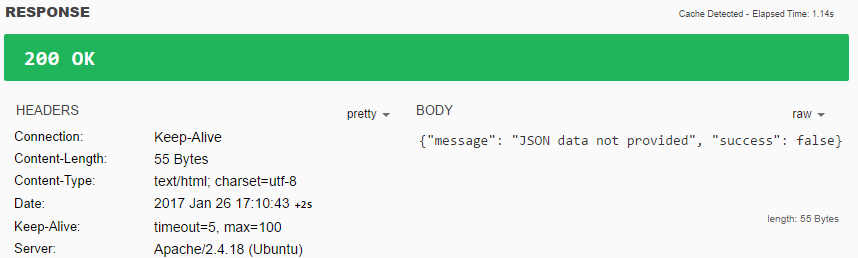
\includegraphics{figs/5/200fail}
    \caption{Screenshot of returned 200 status code}
    \label{fig:msa:200fail}
\end{figure}
\subsubsection{JSON rather than XML}
Both JSON and XML are syntaxes designed to communicate data between the server and the client side browser. Both syntaxes are human readable, hierarchical, can be parsed and used by various programming languages and can fetched using HTTP request.
But JSON outperforms XML in various ways. JSON is shorter to read and quicker to write. JSON uses array lists which provide an efficient mechanism to group all similar data. It also doesn't require a parser to be read by JavaScript programs, so it is much more compatible with front end. The use of JSON format is much simple and less prone to errors as shown in figure \ref{fig:msa:jsonvsxml} \citep{jsonvsxml}.
\begin{figure}[H]
    \centering
    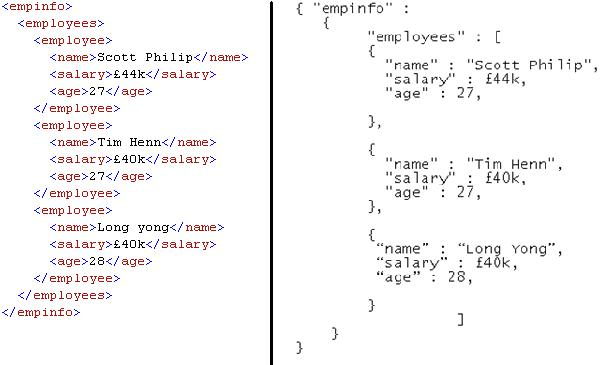
\includegraphics{figs/5/jsonvsxml}
    \caption{XML and JSON syntax format for same given data}
    \label{fig:msa:jsonvsxml}
\end{figure}
\subsubsection{Using JSON with HTTP rather than SOAP}
SOAP (Simple Object Access Protocol) is an XML based messaging protocol which sits on the top of HTTP protocol. HTTP can be considered as delivery truck which transports payload boxes packed by SOAP. Like XML, SOAP has a definite structured rule to follow making it bulky and prone to errors. Sending a JSON data via HTTP is much simpler than sending a XML data using SOAP. Not only that, SOAP is much slower in comparison as it must parse the XML file which it is embedded as payload. \citep{SOAP}
\section{Implementation}
Each micro service is a server running independently on their own personal endpoints endpoints. Flask which is a micro-framework for building python based web-servers, was used to write the server side services code. There is a route () decorator to direct services which internal function to trigger based on a given URL. It also supports WSGI (Web Server Gateway Interface) which provides an interface for back-end server to communicate with application and vice versa. \citep{introduction—wsgitutorial}
Out application implements five micro services: Productizer, Saturn, Olivia and Classifier. It also has 2 external services running as part of front end GUI. Productizer is the main client facing service that allows non-technical user input. It adds images to the SQS queue for image processing which is sends to the back-end by `Grunt' for processing. PubNub provides real time experience to the user by updating the page without having to refresh it. Communication between Productizer, SQS and Grunt take place using HTTP protocol whereas PubNub uses socket communication. This is expanded on in chapter of this report covers in more detail about the technical aspect on how front end GUI works along with two external services to handle multiple data.
All the communication between the front-end GUI and Saturn which is the main back end server, takes place using HTTP protocol (e.g. POST, GET and DELETE). Saturn is the only server that can connect front-end with the remaining two micro-services (Olivia and Classifier).
The Olivia micro-service is responsible for extracting attributes from tiled images, whereas Classifier is responsible for classifying the set of images based on their attributes. Both the servers don't have direct communication with each other. Saturn acts as a main communication tool for both.
To make each service independent and capable of operating on its own, they can handle data in both x-www-form and JSON format. All the services run on a Virtual Machine which operates on Ubuntu 16 Linux Operating System. System runs on Ubuntu because Linux provides an excellent command line command which is every useful when working with remote Virtual Machine using secure shell.
\begin{figure}[H]
    \centering
    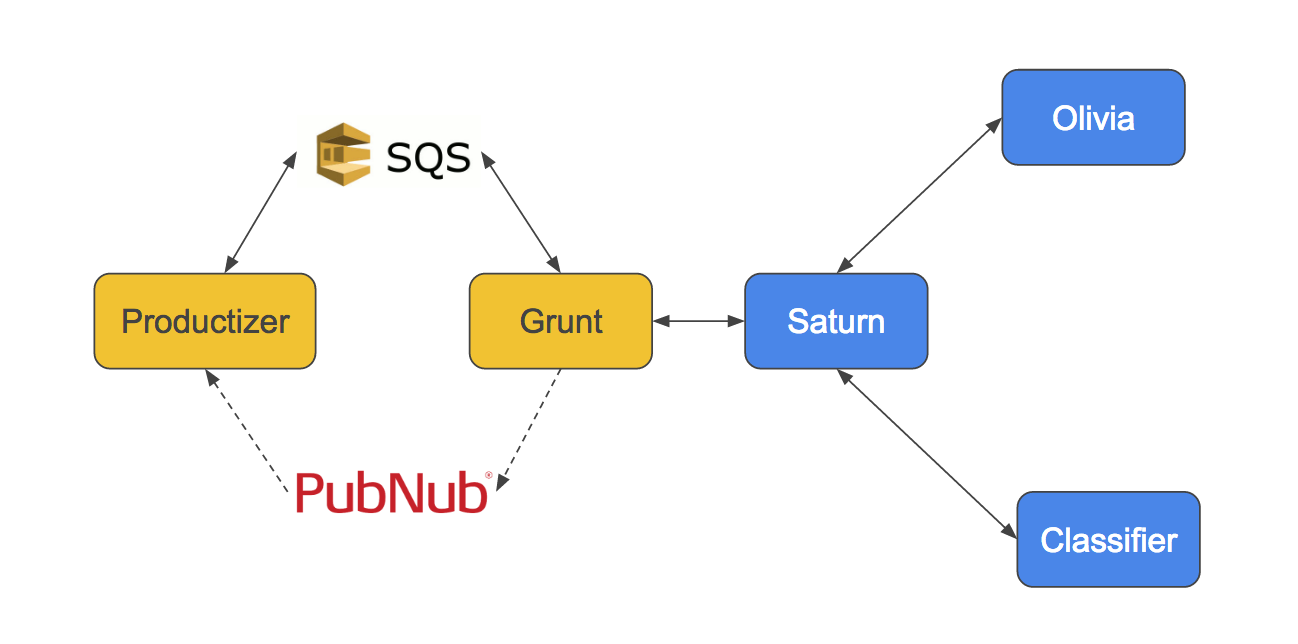
\includegraphics[width=\textwidth]{figs/5/msa}
    \caption{Application Micro-Services Architecture}
    \label{fig:msa}
\end{figure}
In figure \ref{fig:msa}, the double arrow lines represent communicate communication between micro-services using HTTP protocol whereas the dotted lines represent socket communication.
Saturn handles the data first-hand which it receives from front-end GUI. It performs necessary coordination of task in-between the micro-services and returns the data to the front end along with HTTP request status report.
\section{Testing}
For testing purposes, each endpoint was tested to see if it was active and returning the correct data. Each service has many endpoints (assessed by varying URLs), each endpoint has a different function.  So, each endpoint link was being tested to see it works, doesn't break and give out correct output using DHC (Div Http Client). DHC is an HTTP Client, well suited for API testing of multiple services. Figure \ref{fig:msa:200fail} is an example of end-point test result using DHC.
\section{Limitation}
Despite all the benefits of micro-services it is accompanied with limitations that cannot be ignored. Deploying a single application by decomposing it into multiple small services increases maintenance responsibility such as building, testing, deploying and running. Having multiple services means there must be a uniform way to communicate in between them by introducing an interface. Both sides need to exchange messages using same format and should have same understanding of message semantic.
Micro-services can be considered as a distributed system which means all the problems that exist within such system has be considered (e.g. network latency, fault tolerance, message serialisation, etc.) \citep{microservices-notafreelunch} It also increases the resource use as each service is running independently using their allocated processing power and memory. It also requires continuous monitoring as each service need to be up and running for the whole application to work. These are some of the limitations that need to be considered.
\section{Evaluation}
Micro-services architecture provides the agility to replace and update any components within the overall application. Each service can be built using the most appropriate tool for the task. Each service is small fraction of a much larger system, which can worked upon independently and at different point of time. The whole system is loosely coupled which eliminates the susceptibility of a single point of failure. In conclusion, this architecture provides this ability to work on a single application by group of people without having to worry about how the whole system works.



\chapter{Productizer} \label{chapter:Productizer}

\section{Overview}

Productizer is the user-facing web application that handles everything from the initial uploading of aerial images, slicing the image into tiles, and enabling user communication with the ‘back-end’ services of the project in order to teach and retrieve classifications from the classifier. The application is PHP-based, built upon the Laravel 5 framework and utilises Bootstrap as a front-end framework. Throughout the development of Productizer, there was a heavy focus on ensuring that the user experience was as practical and elegant as possible. There are 3 main steps to the system: uploading an image, learn mode and discover mode.

\section{Design Decisions}

\subsection{PHP Framework}

Having selected PHP for the web application, the choice was made to use an MVC framework. The framework selected for this was Laravel, a largely popular MVC framework amongst PHP developers due to it’s abundance of out-of-the-box features such as built in queue handling, authentication systems and built in protection against a large number of web vulnerabilities. It also provides great utility when using the MVC design pattern, separating the ‘business logic’ from the ‘presentation code’. 

\subsection{Tiling and Google Maps API}
One of the first design decisions that had to be made was how to display the uploaded image to the user whilst incorporating required features, such as region selection within the image. Google Maps provides a comprehensive API that supports a large number of desired features for the final product. One major reason for choosing this API was that a fixed tile size could be selected and used by the API to render the map. This seemed to link in very well with how the attribute extractor was designed as it required the input to be a 256x256px image, meaning that the same images could be used to render the map and could be selected by the user to send to the back-end services. As well as this, the API provided all the same features that can be used on Google Maps such as pan and zoom, plus allowed the ability to draw polygons and place markers on the map, meaning that user selection could be displayed in an elegant format.

\subsection{Queue Driver}

Another design decision that had to be made was what queue driver to use within Laravel in order to store and handle jobs. Included with Laravel are a number of different queue drivers, including databases (all jobs are stored in a database table), Amazon Simple Queue Service (SQS) and Redis. Due to the use of a microservices architecture, the approach of using an external service to provide queue support was preferred. Amazon’s SQS was therefore selected due to it’s quick setup and robust infrastructure.

\subsection{Publish-Subscribe Service}

Within the web application, the decision was made to use a real time publish-subscribe service, allowing changes to be made to the user interface without the user needing to refresh the page, based on messages sent along a specific channel. This meant that a queue handler could directly communicate with any running instance of the web application to inform it of any relevant data that had been processed, allowing these instances to update accordingly. A commonly known real time publish-subscribe service is PubNub. PubNub provides SDK’s for an impressive number of programming languages, and currently parses over 1.8 trillion messages every month \citep{pubnub_2016}. We mainly made our decision to use PubNub due to it’s support for both PHP and JavaScript, along with it’s impressive low-latency during transmission of messages.

\section{Implementation}

\subsection{Uploading Images}

The first step that a user will take when using the application is uploading an image from their own computer. The application allows a user to upload an aerial image in TIFF/JPEG format (typically 4000x4000px), which is then processed, generating tiles that are used throughout the rest of the application. The image, and every tile generated from it, are also assigned with unique ID numbers. The application also provides a history of past uploads that allows any user to recall images that they have worked on in the past.

\subsection{Tile Generation and Fuzzy Borders} \label{section:fuzzy}
Initially, the system’s tile generation split each uploaded image into 256x256px tiles which were then displayed as a “map” using Google Maps API. In this first design iteration, user selection was limited to each of these distinct tiles meaning that the application suffered from a ‘fuzzy borders’ problem. Fuzzy borders is an issue where a user is attempting to select a certain feature, but with selection limited to a fixed grid the feature may lay across the border of two tiles, meaning they are unable to select that feature. This can be seen below, in figure \ref{fig:prod:fuzzyold}.


\begin{figure}[H]
    \centering
    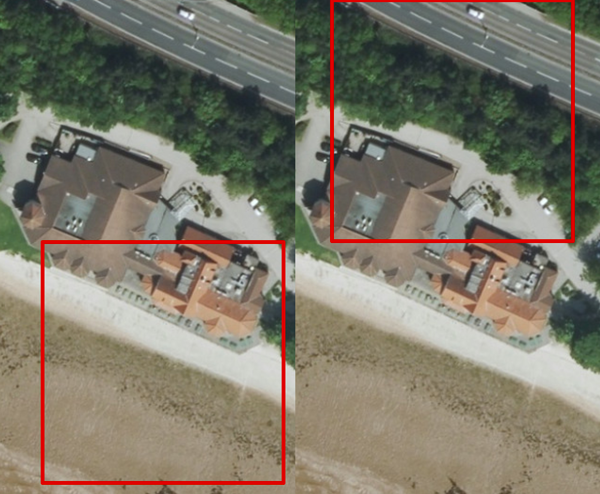
\includegraphics[width=\textwidth]{figs/6/fuzzy-old}
    \caption{With a fixed 256x256px grid, the house that a user wants to select crosses the border of two tiles, so they are unable to select it.}
    \label{fig:prod:fuzzyold}
\end{figure}

To combat this issue, instead of just splitting the image into 256x256px tiles, it was split into 128x128px tiles, and these smaller tiles would act as `selection tiles’ for the larger tiles. The larger tile would contain the smaller `selection tile’ in the top left, with it’s neighbouring tiles filling in the rest of the larger tile. The 128x128px tiles were then used to display the map using Google Maps API, however when selecting one of these tiles, it’s larger counterpart would be the area that actually was selected. This effectively meant that the system moved from a 256x256px selection grid to a 128x128px selection grid whilst maintaining a 256x256px selection size, effectively quadrupling the selection space. With this new system, the user is able to select an area that was previously split between borders of tiles, helping remove fuzzy borders. The result of this as compared to figure \ref{fig:prod:fuzzyold} can be seen below in figure \ref{fig:prod:fuzzynew}.

\begin{figure}[H]
    \centering
    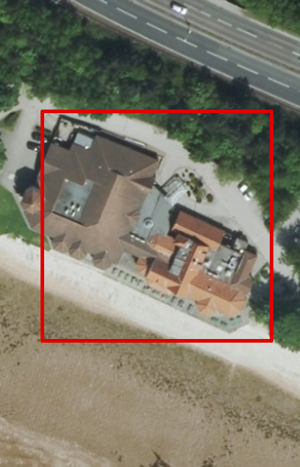
\includegraphics[width=8cm]{figs/6/fuzzy-new}
    \caption{With a 128x128px grid, and 256x256px selection, a user can now select a house that used to lay in the middle of two tiles.}
    \label{fig:prod:fuzzynew}
\end{figure}

\subsection{Learn and Discover Mode}

Having completed the processing of the initial image, Productizer provides two modes to the user: learn and discover. Learn mode provides a method of supervised learning for the classifier, allowing users to select a number of different tiles and a certain class before submitting. These are then sent to Saturn, which in turn provides the classifier with supervised training data generated from these tiles. The classes of the system are displayed in a dropdown, having been retrieved from Saturn, and there is also the ability to add new classes to the system within learn mode. Once the user has finished with learn mode, they are able to switch to discover mode by flipping a simple toggle switch.

Discover mode allows a user to select and filter which class(es) they wish to discover, and markers are added to the map for each tile that matches a selected class, with distinct colours to represent each class. Upon hovering on one of these markers, the class name is also displayed in a simple text bubble. The initial classification is automatically generated upon the initial upload of the image, with every distinct 256x256 tile being sent in batches to Saturn in order to retrieve a classification that is then stored in the database. Every time learn mode is used however, these classifications become outdated, so discover mode also provides the ability to re-classify every tile upon the click of a button, updating this classification data. Storing these classifications inside of a database for each unique tile essentially caches the results, optimising load time.

\subsection{Amazon SQS}

The first design iteration would simply create a GET request containing all of the tile image URLs, and submit this to Saturn manually for reclassification. This proved to be very inefficient as the request size was large, while server processing and thus response time was slow, and if a request was lost due to network issues or some other means, the user could end up waiting a large amount of time for no reason. To combat this, a queue system was implemented within the application that utilised Amazon Web Service’s Simple Queue System (SQS) to store and handle different jobs that were to be completed. In order to handle the retrieval and submission of these tasks, a new task worker, ‘Grunt’, was introduced as explained below. Storing these tasks with SQS meant that a smaller request could be sent to SQS to store the processing data, and then the user could be presented with a processing page until every item in the SQS queue had been processed so that they were aware of what was happening behind the scenes while waiting for their new classifications to be displayed. Furthermore the queue worker enabled retries to be handled if a request fails, delegating responsibility of ensuring the job is completed to the queue worker as opposed to the user. This new implementation greatly boosts user experience.

\subsection{PubNub}

One of the goals with the new processing page was for the user to be informed of the processing results in real time, without the need to constantly refresh the page to check the status of processing. This would mean that, as well as improving user experience, it would reduce server load in the scenario where a user would constantly refresh the page. In order to achieve this goal, a publish-subscribe mechanism was implemented with PubNub. The ‘topic’ used for PubNub would be a unique map ID, allowing the queue worker to publish on to this topic every time a new tile batch had been processed. The Javascript code within the map display page would subscribe to this topic, and every time a message was received informing it that a new batch had been processed, the user interface would be updated to reflect this. This real-time data transfer meant it was possible to display a live loading bar, and iteratively add map markers to discover mode as new tile classifications are received.

\subsection{Grunt}

Grunt, the queue worker, utilises Laravel’s built in job and queue functionality. Out of the box, Laravel enables the use of Amazon SQS as a queue driver, meaning implementation was greatly simplified. In order to create a job type, a specific job class needed to be build, that was named BatchProcessTile. The tile generation process was responsible for defining batches of tiles, and passed through a collection of tiles to each new job. The implementation with SQS operates by serializing the job object once it has been constructed and sending this to Amazon’s servers. Once Grunt retrieves this queue object, it is deserialized and the `handle’ method of the job is called. Within the `handle’ method, the collection of tiles is formed into a request that is sent to Saturn, with a retry handler that takes care of re-sending failed requests. Once an accepted response is retrieved from Saturn, containing the re-classification data, the `handle’ method updates each tile from the batch, storing it’s new classification in the database. Once this has been completed, it publishes a completion message to PubNub as explained above.

The decision to create Grunt as a separate microservice arose early on in project testing when the back-end was not making use of the GPU, so responses took a lot longer to receive than they do in the current iteration of the application. At this stage, Productizer would simply send all requests itself directly to Saturn in order to retrieve the result, which took 5 minutes or more for the response to be received, whilst all the user would see was a white screen with a loading wheel in their browser. This is a dreadful user experience, and from testing it was revealed that users would often refresh during this process, which would reset the waiting time and put more strain on the server. By implementing Grunt, the user was taken to a processing page as soon as the image had been uploaded, so they were informed with exactly what was going on via a loading bar indicating progress. Despite this problem being much less severe now that the back-end makes full use of the GPU, it helps mitigate other potential issues that could have arisen during this process, such as network issues that might have caused a request to be interrupted, putting responsibility on Grunt to complete the task.

\section{Testing} \label{section:prod:testing}

Testing was heavily integrated within the development of Productizer. As the focus during development was heavily based around user experience (UX), the testing was tailored towards this. Functional testing, look and feel testing and usability testing were all carried out to ensure the UX of the application was optimal. 

\subsection{Functional Testing}

The functional testing set out to ensure all buttons/GUI elements behaved as expected. This involved making sure links lead to the correct locations, the correct results were obtained from certain stages of the application, and the overall functionality of the system worked as intended. No formal documentation was created for this testing, as with every new iteration of Productizer, the entire process of the system was tested from the start, meaning that every aspect of the site was checked during each iteration. 

\subsection{Look and Feel Testing}

One key part of optimising UX for the user was the look and feel testing. With this, it was important to ensure that the process of using the application was enjoyable and straightforward. To check this, external feedback was required, so throughout the development lifecycle, colleagues were asked to navigate around and use the application, and provide feedback. Additionally, one fantastic component of scrum was the weekly meetings with Izzy, providing direct UX tests with the client every week, allowing for adjustments to the UI and UX based upon her feedback in time for the next sprint.

The most noticeable change to the UX that arose from look and feel testing was the migration from using a small area for the map with the controls down the side, as shown in figure \ref{fig:prod:olddesign}, to having a much larger full width map, with the controls underneath, as shown in \ref{fig:prod:newdesign}. One colleague had a much larger resolution display compared to the devices used for development. With this, they identified a problem where workflow could potentially be slowed due to such a restrictive map area. Following this feedback, a full screen map layout was developed, and other colleagues and Izzy were asked which layout they preferred. The result was unanimous in favour of the fullscreen layout, so this became the new design.


\begin{figure}[H]
    \centering
    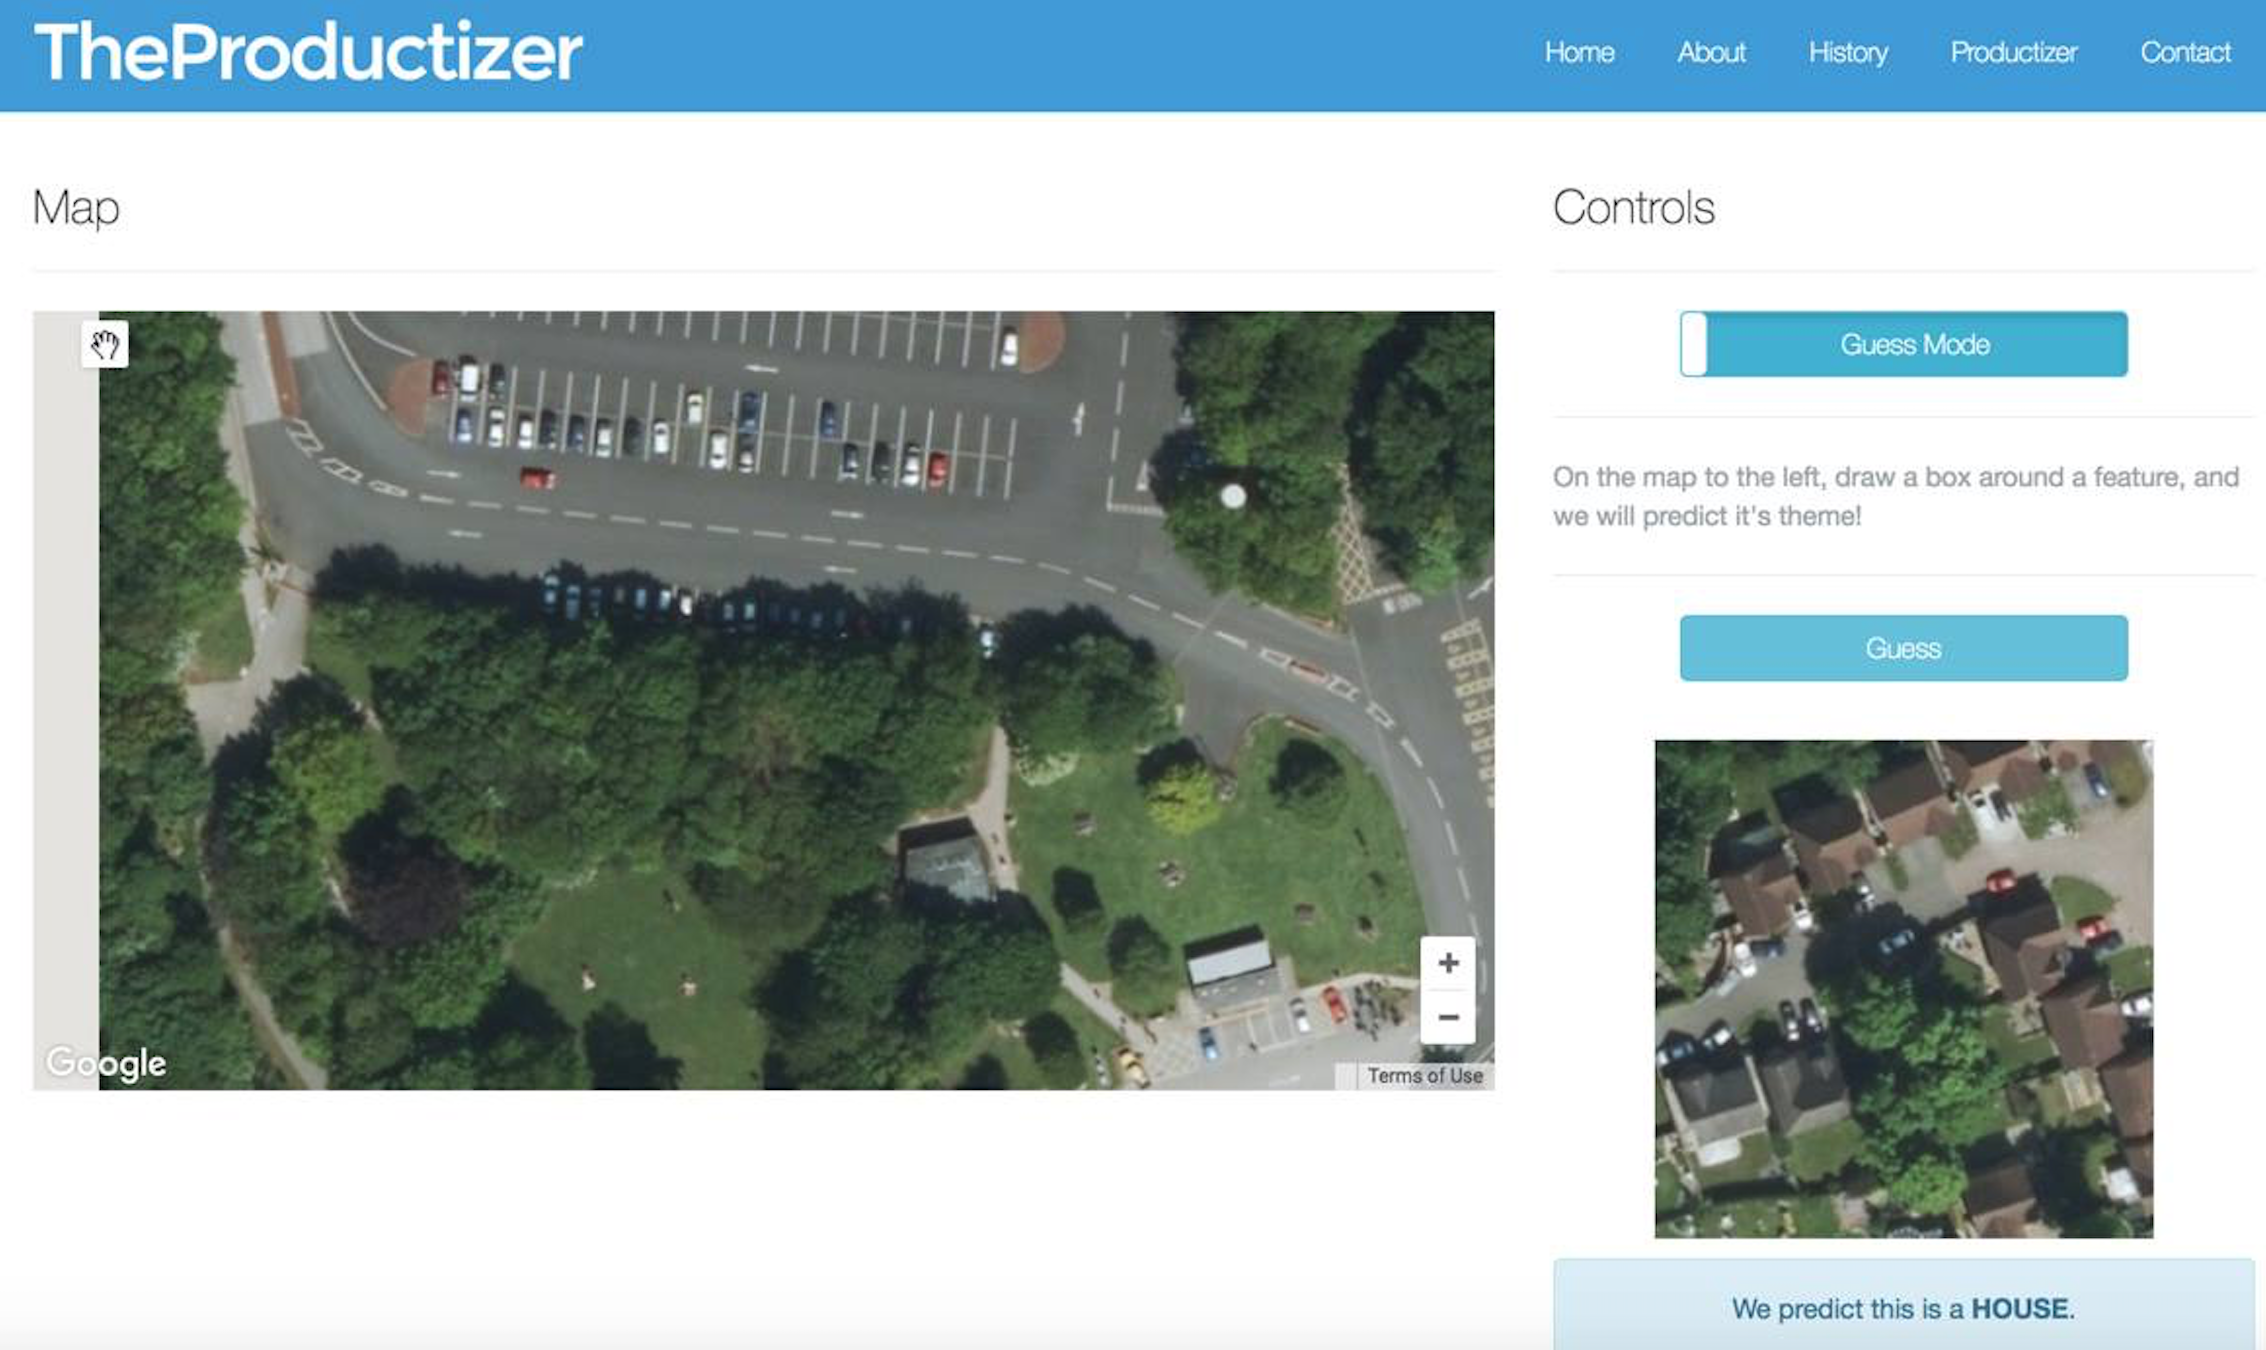
\includegraphics[width=\textwidth]{figs/6/6-testing-olddesign}
    \caption{The initial Productizer design, with small map interface and controls along the side.}
    \label{fig:prod:olddesign}
\end{figure}

\begin{figure}[H]
    \centering
    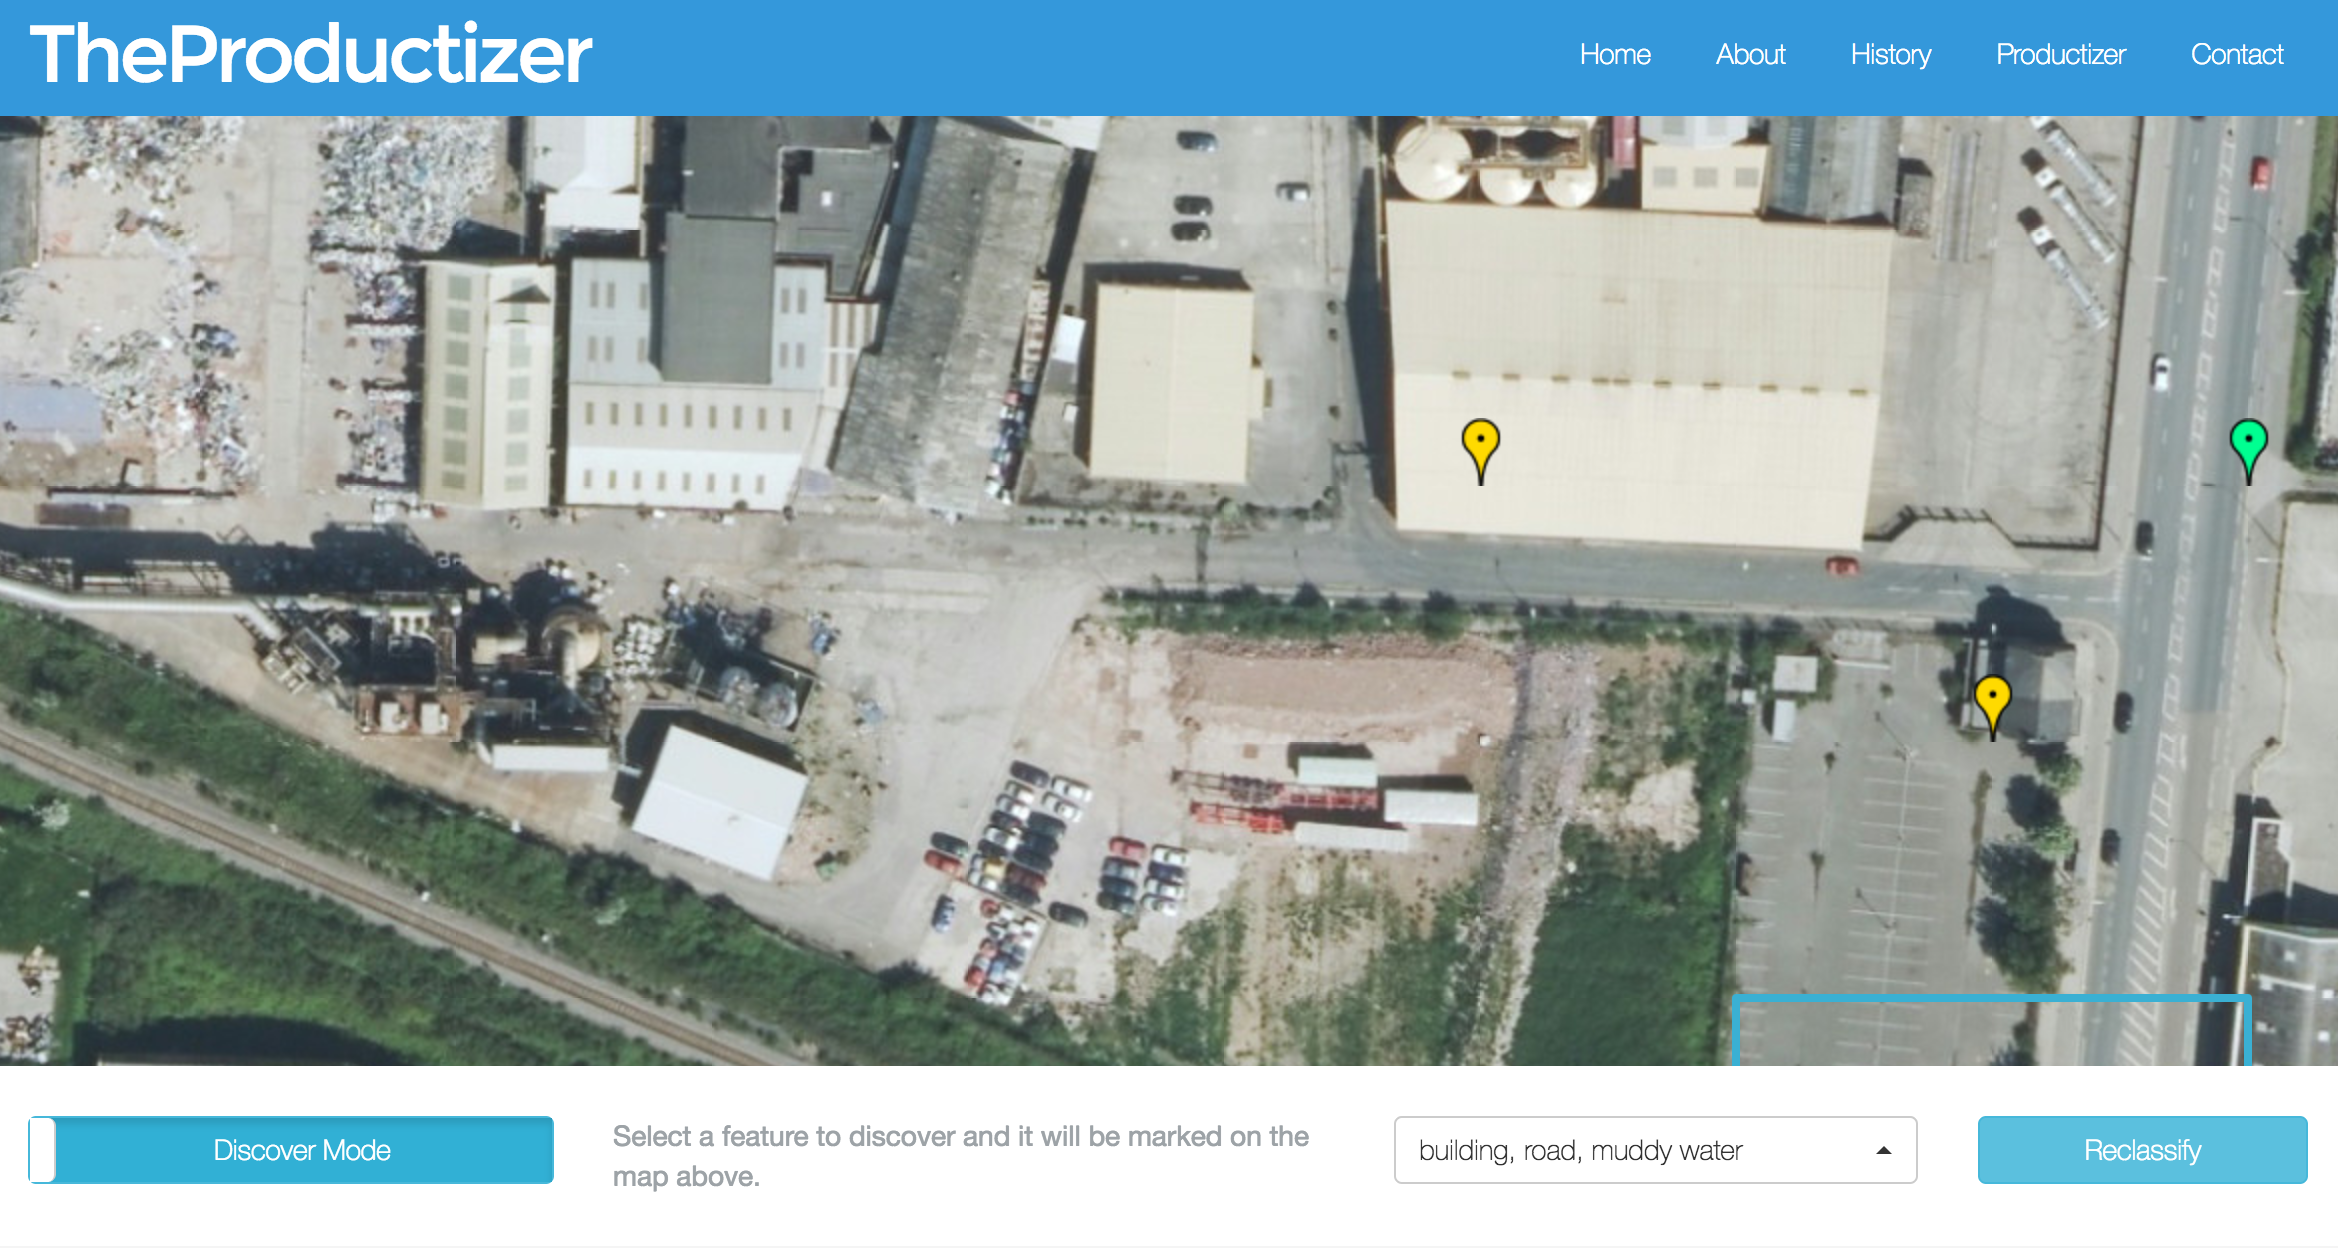
\includegraphics[width=\textwidth]{figs/6/6-testing-newdesign}
    \caption{The revised Productizer design, with full width map interface and controls along the bottom.}
    \label{fig:prod:newdesign}
\end{figure}



\subsection{Usability Testing} \label{section:productizer:usability}

Usability testing involves sitting a user down with the system and running them through a specific process to test ease-of-use and identify confusing features or features that could be improved.

As mentioned in the above implementation, one issue identified early on during usability testing was the initial loading time during the uploading and processing of the image due to the communication to Saturn, that could take anywhere up to 5 minutes or beyond. Upon identifying this problem, research was carried out into typical response times and their effects on the human brain. \cite{nielsen_1993} found that a 0.1 second response was considered an “instantaneous response”, a one second response was the limit of maintaining a user’s flow of thought, and ten seconds was the limit of keeping the user’s attention. This article also stated that in a situation where instantaneous feedback cannot be provided to the user, a “percentage-done” indicator should be used. The original plan was to optimise the loading time to be within this 10 second limit of attention, however within the time constraints of the project this was not a viable aim, so a “percentage-done” indicator was implemented as suggested, and can be seen below in figure \ref{fig:prod:loading}.


\begin{figure}[H]
    \centering
    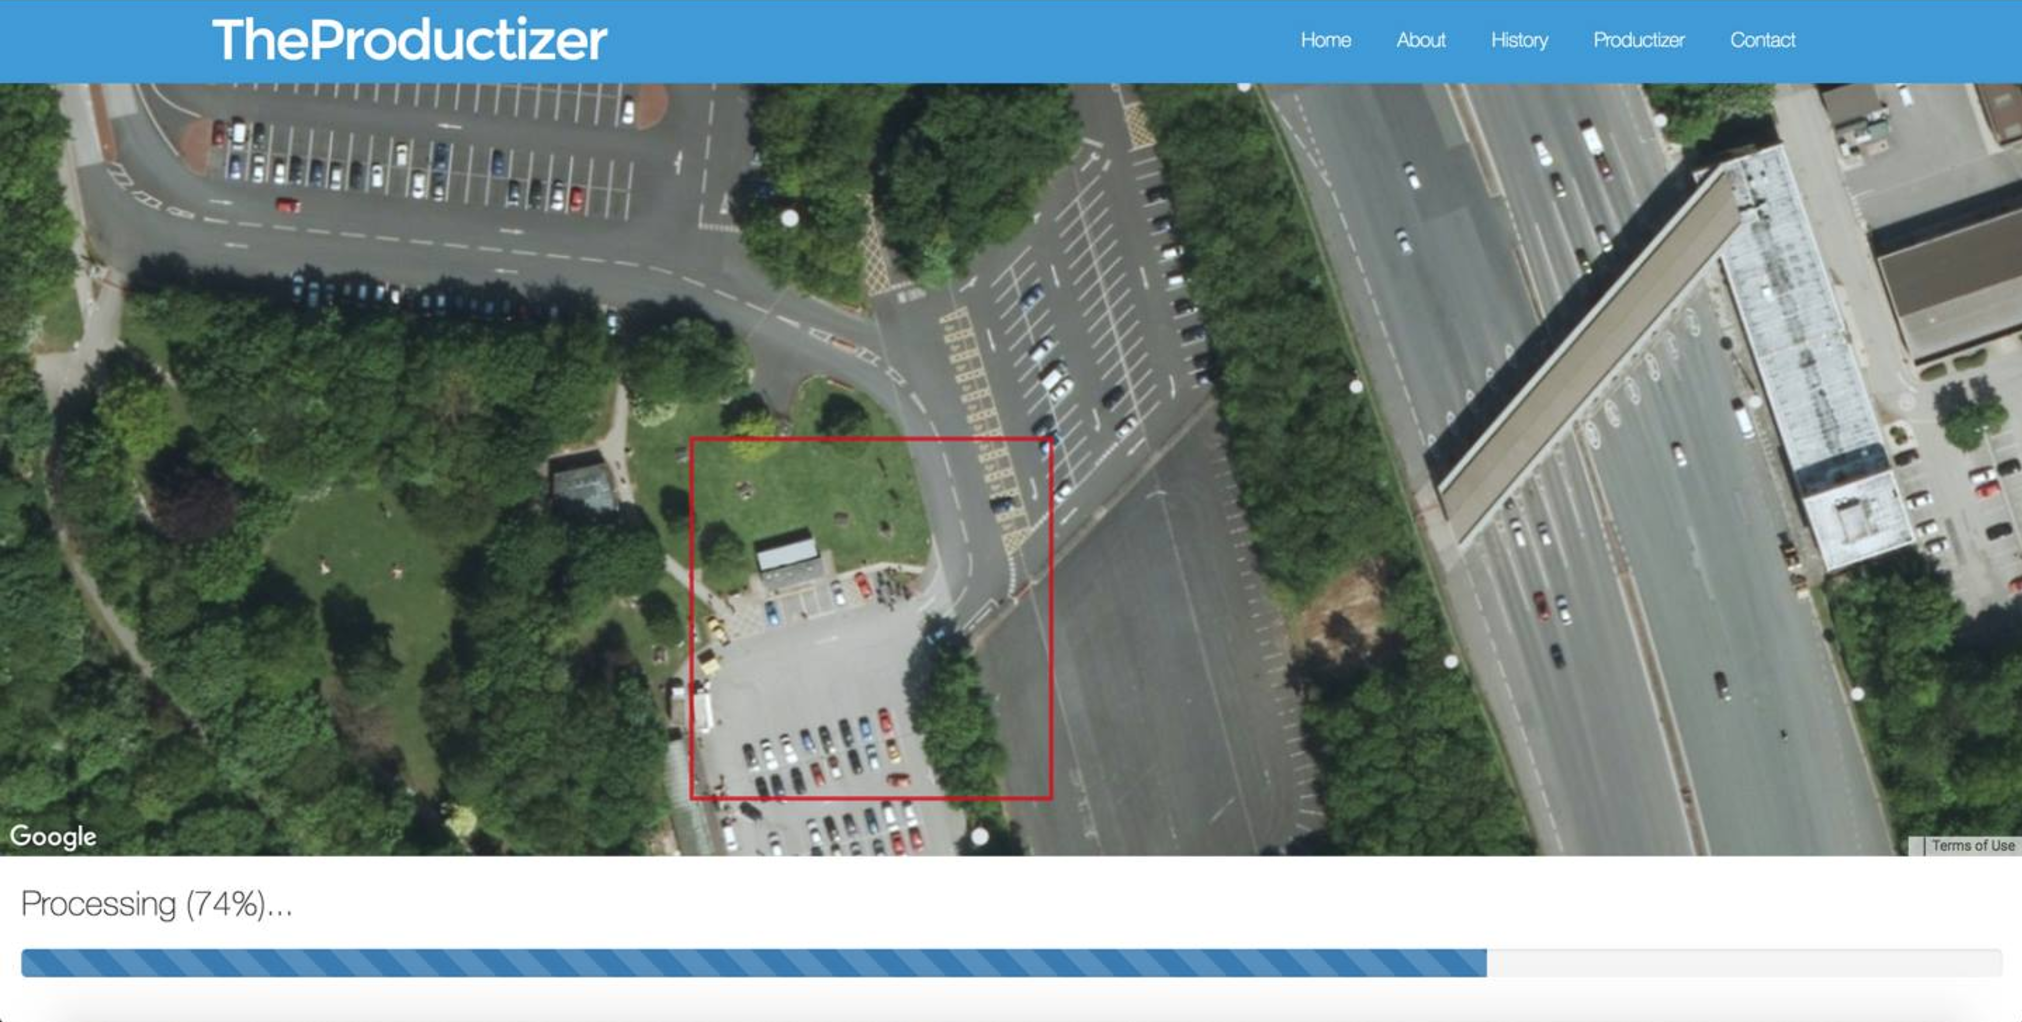
\includegraphics[width=\textwidth]{figs/6/6-usability-loading}
    \caption{A percentage-based loading indicator provides the user feedback of processing percentage.}
    \label{fig:prod:loading}
\end{figure}

Final results of the usability testing conducted with Ordnance Survey can be seen in the results section further on in this report in section \ref{chapter:results}.

\section{Limitations}

A limitation found during testing Productizer was the time that it takes for a user to upload an image to the system. Most sample images provided by Ordnance Survey were around 40 to 50MB in size, and these images could take a significant time to upload if the user’s upload speed was slow, and lead to additional issues should the user’s network be unstable. Unfortunately this is an external limitation that cannot easily be optimised within the scope of this project. However, the images provided by Ordnance Survey were of TIFF format which, when converted to JPEG, were much smaller in size (around 4 to 5MB) without significant loss in quality, so it may be quicker to convert the TIFF images to JPEG format before upload, should the user have a slow connection.

\section{Evaluation}

The user-facing web application, Productizer, was designed to be a solution that allows a user to upload an aerial image and, through a streamlined process, manipulate and select regions on a map in order to train a classifier, and obtain its predictions to discover features similar to those used in training. Following the three required features of the web application outlined at the start, Productizer is now a complete solution for this design, with a heavy focus on optimising the user experience through this process. A user can upload an image, and can then select a number of different tiles to be used to teach the system. Following this, they can use “Discover Mode” in order to identify and filter different features identified on the image that they have uploaded. The design is mobile-optimized too, allowing for flexibility in its use across multiple devices.
\chapter{Olivia} \label{chapter:Olivia}

\section{Overview}
Olivia is the microservice responsible for extracting attributes from an image, named after Olivia Wilson as the technology used in the service utilises her work done during her Masters project. Note that all references to ‘Olivia’ are referring to this microservice. Taking Olivia from a black box perspective, it take a 256 by 256 pixel image and returns a corresponding attribute vector (of 1024 elements) that `describes’ the image. 


\begin{figure}[H]
    \centering
    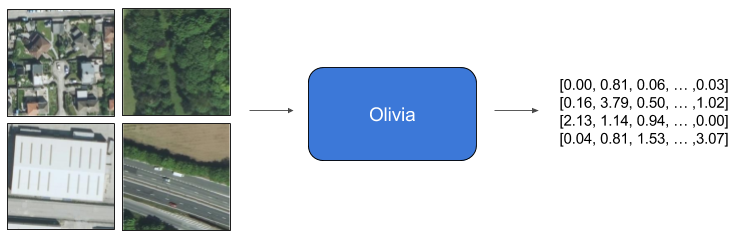
\includegraphics[width=\textwidth]{figs/7/olivia-goal}
    \caption{Visual Description of Olivia}
    \label{fig:basic_olivia}
\end{figure}


Attribute extraction for images is a complex task, and there are many questions that need to be asked. How attributes should be extracted from images? How many attributes should be extracted? What attributes are necessary to distinguish each image uniquely? How do you determine when a feature starts and finishes? Wilson’s work answers many of these questions, but also introduces others, some of which are solved in this project. 

This microservice was designed to act as both a standalone service and module within a system (like this project). It has its own HTTP endpoints, persistence and control sequences, all of which allow it to be used independently from the other services in the system.


\section{Background Research}

\subsection{Terrapattern}

Terrapattern (discussed in section \ref{section:existing:terrapattern}) evidently has a fantastic attribute extraction module. It has an impressive ability for recognising edge cases, and despite often finding differences between images that a human would believe to be identical, this only provides further evidence that it can extract a vast number of attributes to identify such subtle differences. 

On further inspection of the public source code (\url{https://github.com/CreativeInquiry/terrapattern}), it seems rather evident that there is a private side to the repository that the website is using. The code available uses six different languages and the submodules contained are written in an additional three languages. Despite being open source, the codebase seems so obfusticated that it is unusable. 

\subsection{Wilson’s Work}

Wilson’s paper, entitled ``Incorporating scale into convolutional neural networks for use on aerial image interpretation” and commissioned by OS, looks into extending a deep neural network to increase image classification of map tiles. This new neural network (now 17 neural network nodes) accepts a 256 by 256 pixel image and classifies the centre pixel based on the surrounding 192 by 192 pixels (as can be seen in figure \ref{fig:olivia_range}). As this project and ours are commissioned by OS, the code is available with assistance from Wilson and others.

\begin{figure}[H]
    \centering
    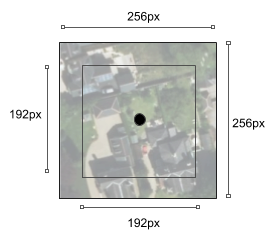
\includegraphics{figs/7/tile_range}
    \caption{Olivia Classification Visualisation}
    \label{fig:olivia_range}
\end{figure}


\section{Design}

Olivia has a single responsibility: to extract attributes when provided with map tile images. While this can be a slow process, it has been optimized in order to fulfill this responsibility without significantly impacting the user experience. The main case flow is quite simple: when given an image, check if the image has been seen before. If so, return the vector previously computed. Otherwise, convert the image to an attribute vector, remember it and return the vector. 

\begin{figure}[H]
    \centering
    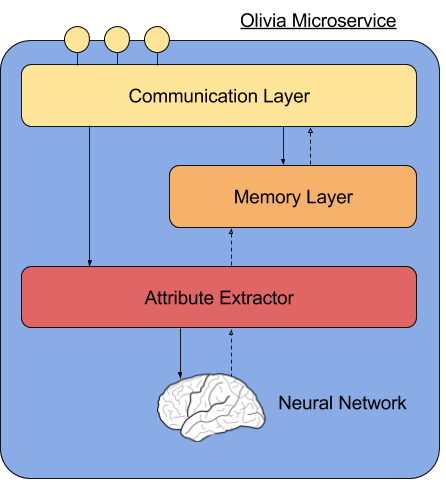
\includegraphics[width=8cm]{figs/7/olivia_design}
    \caption{Olivia Microservice Design}
    \label{fig:olivia_design}
\end{figure}

A number of decisions had to be made when considering the design and implementation of this mircoservice:

\subsection{Wilson’s Code or Terrapattern}

Having seen Terrapattern’s website, it looked like a prototype that could have been extended to match the requirements of the project. However as mentioned in section \ref{section:existing:terrapattern}, the code was unusable and included using experimental languages. 

Wilson’s code, in comparison, could be deconstructed to use the trained deep neural network (DNN) for attribute extraction. Originally, the network produced four outputs, corresponding to the probability of the image belonging to four major themes. The number of nodes in neural networks diverge as they reach the centre of the network and then converge towards the output layer. To increase the output of Wilson’s DNN, we removed the last four layers resulting in an output of 1024 non-negative doubles that are the decomposition of the image (shown in figure \ref{fig:NN_decomp}). Due to the issues with Terrapattern, the use of Wilson’s code was chosen. 

\begin{figure}[H]
    \centering
    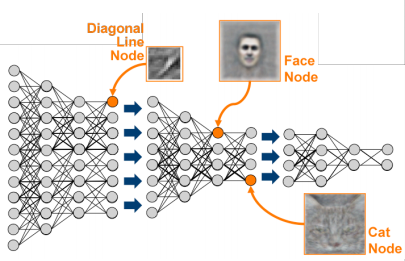
\includegraphics[width=12cm]{figs/7/NN_decomp}
    \caption{A visualization of a NN classifying images \citep{murnane_2016}}
    \label{fig:NN_decomp}
\end{figure}
	
\subsection{GPU or CPU}

The DNN produced by Wilson runs on a nervana module that works on tensor flow. This supports uses the processor or graphics card to compute the output of the DNN. Comparing the two, the processor is easy to setup and easier to maintain. Using the graphics card is complex and somewhat unreliable. Under experiments, the CPU processed one image every 30 seconds, whereas the GPU completed 128 images every tenth of a second. The speed of CPU prevented it from being a viable solution hence GPU processing was chosen. 

\subsection{Wilson Ignores Border Issue} \label{section:nsew}

As can be seen in \ref{fig:olivia_range} (page \pageref{fig:olivia_range}), Wilson’s DNN ignores the 32 pixel border, which makes up 43.8\% of the 256x256 tile. This information could be deemed important to another module, depending on circumstance. 

\begin{figure}[H]
    \centering
    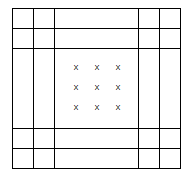
\includegraphics[width=5cm]{figs/7/NSEW_points}
    \caption{NSEW Approach}
    \label{fig:NSEW}
\end{figure}

A method, nicknamed “North, South, East, West” (NSEW) within the project, proposes to shift the 192 pixel focus 32 pixels in each direction to ensure full coverage of the image (as shown in figure \ref{fig:NSEW}). This produces 9 points of focus around the centre of the image, producing 9 attribute vectors per image. The result of this is that every pixel in a tile is covered, with an extra 93\% contextual data gathered from the overlap. This means that every classification decision is made using more information about its surroundings, improving the accuracy. A comparison of the two methods can be observed in figure \ref{fig:NSEW_cover}.


\begin{figure}[H]
    \centering
    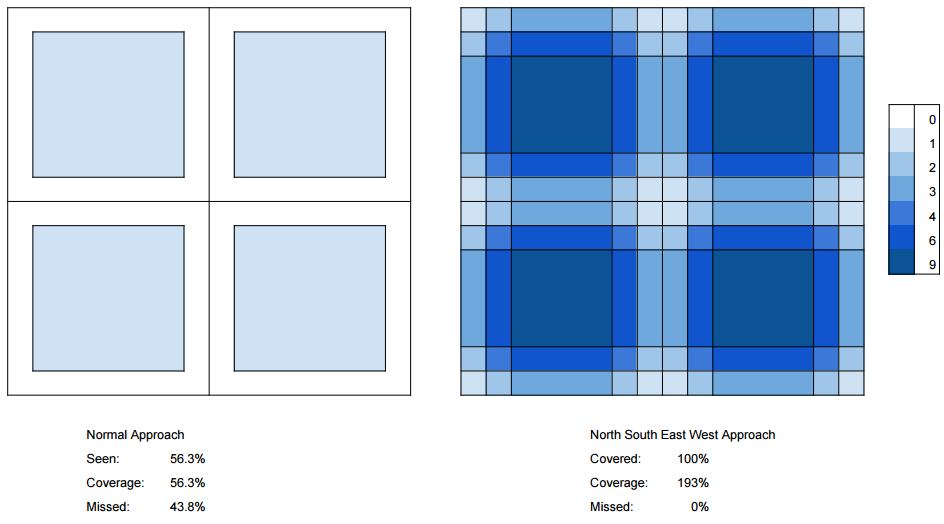
\includegraphics[width=12cm]{figs/7/NSEW}
    \caption{Coverage of NSEW Approach}
    \label{fig:NSEW_cover}
\end{figure}

\section{Implementation}

The core of the modules implementation uses Wilson’s code as a black box. However, to achieve the design, a control or logic layer needed to be included, which required subtle adaptations to the service. These changes will be discussed by the order in which they are used in the flow of the entire system. 

When testing the system, a key bottleneck was downloading the images. This would take considerably longer than processing. Therefore to compensate for this, a new endpoint was introduced ``\textless{}olivia\textgreater{}/download”, which simply accepts a dictionary of image URLs and their tile\_id. Tiles are identified by: \textless{}map\_number\textgreater{}\_\textless{}x\_pos\textgreater{}\_\textless{}y\_pos\textgreater{}. This enabled the service to convert the image on demand rather than waiting for the image to download and convert. This does not reduce the time for the entire process, however through observations of user interactions it was found that the user will not request conversions for considerable time. This time is utilised by downloading the images, as this will occur when they ‘discover’ features later.

The next most expensive operation in the system is the attribute extraction. An observation about this is that no matter how many times you convert an image, the vector returned is always the same, because the DNN  never changes. Therefore once an image is converted, the result can be stored to reduce the best case and average time complexity of conversions to 1, significantly reducing the overall time for a full ‘discover’ sweep.

The first iteration of the service offered the standard convert and the NSEW convert. Both would perform as expected, where the standard convert would perform one conversion per image and NSEW would perform 9 per image. However it was found that the even when a standard convert was requested, the NSEW convert would be requested soon after. Hence in iteration 2, the standard convert would perform the NSEW convert and simply return the middle attribute vector. This reduced the overall computations during the ‘discover’ sweep (that uses NSEW convert). Additionally, since standard converts were often less than 14 images (and 14x9=126 conversions), this would not increase the processing time for standard converts, since 128 conversions can be performed concurrently, explained below. This way the service can extract more data in the same amount of time. 

As the GPU was considered the optimal method for processing extractions, batching had to be managed. Through incremental testing, it was found that 128 concurrent conversions was the perfect balance of stability and performance. This is then complicated by the NSEW approach, as this increases the number of conversion $n$ to $9n$. Ensuring that all nine attributes vectors of an image succeed or fail together is essential to prevent corruption of results. Therefore, a maximum of 14 images can be processed in a single batch, since each image is processed 9 times under NSEW conversions, resulting in 126 conversions with 2 redundantly unused slots.

\section{Testing}
As the system’s most critical sub-module was Wilson’s DNN, this was the first test. To ensure it was behaving correctly, a test image with a known result was passed through to ensure that the expected results match the actual results, on both the last and fourth from the last layer. These unit tests would imply that the DNN has remained unchanged and the modules using it are uncorrupted.

As mentioned, GPU processing was somewhat unreliable with functioning code. To ensure the code was in an optimal state, the batching was unit tested as well as system tested. Other system tests included the NSEW approach, which used test images with coloured 32x32 pixel areas, moved around the image to ensure each of the 9 sections attributes changed only when the coloured area was in their section(see figure \ref{NSEW_test_image} for an example). It was also hand tested to check that a pure white image would provide the same results as sections that couldn’t see the coloured area. There was also a system check script created to run manually to ensure that the GPU processing was configured correctly.

\begin{figure}[H]
    \centering
    
\includegraphics[width=5cm]{figs/7/NSEW_test_img}
    \caption{One of the images used to test NSEW Conversions. The red 32 by 32 pixel squares should only change the results when the focus is shifted to the corners}
    \label{fig:NSEW_test_image}
\end{figure}


\section{Limitations} \label{section:olivia:limits}
The GPU in the machine running Olivia was a Nvidia GTX Titan X with 3072 cuda cores and 12 GB of dedicated RAM. In theory, Olivia should be able to process at least 256 images concurrently, but the amount of RAM proved to be the limiting factor in this instance due to the size of all the images. Therefore, 128 were processed concurrently, halving speed of the attribute extraction.

The minimum tile size is 192 by 192 pixels, which covers quite a large area when using OS’s images. This prevents it from extract attributes about a single feature, since each tile often contains a number of features. For example the data extracted would be correspond to several houses, rather than a single house. 

\section{Evaluation}
This microservice matches the specification; it accepts a tile image and converts it into a collection of attributes. Based on the results seen in chapter \ref{chapter:classifier}, Olivia produces useful attributes. The use of Wilson’s DNN is an evident success. 

Through the discussed techniques, the service has been optimized to reduce the average time required for the full ‘discover’ sweep of the feature finder. These methods, without reducing the time complexity of the service, manipulate the subtleties of usage to pro-actively perform computations when not in demand, and to pause these computations to provide their results when in demand. 

\section{Further Work}
The current NSEW approach results in 9 computations rather than 1. This could be reduced to 5 by only requesting the North East, North West; South East, South West and centre attribute vectors to be produced. This would still cover every pixel of an image, and reduce the computation by roughly half, at the cost of with less accuracy. Experiments could be made to test both extraction methods and determine over an expansive dataset if the tradeoff of reduced accuracy for faster computation time is viable.

A more dramatic improvement would be to entirely retrain the DNN on smaller images. This would allow a more precise feature extraction to occur, combatting the issues mentioned in the limitation section previously (paragraph 2, section \ref{section:olivia:limit§s}). With this there might be less attributes, however the precision gained (through smaller images) would outbalance the negatives.
\chapter{Classifier}
\section{Overview}
The classifier`s task is to solve the following problem: given a vector of 1024 attributes, determine which feature this vector represents. To solve this problem, the classifier must identify patterns in the attribute vectors extracted from features of the same type, and use this to distinguish them from other features, much like a fingerprint. 
Figure \ref{fig:spark_problem} shows a visualisation of these ``fingerprints" in a spark diagram. This diagram shows each 1024 attributes extracted from 20 features. Each row represents a feature, and each vertical bar represents the value of that attribute of that feature
Figure \ref{fig:spark_solution} shows how subtle patterns can be found within these ``fingerprints" that can be used to identify the feature they were extracted from
\begin{figure}[H]
    \centering
    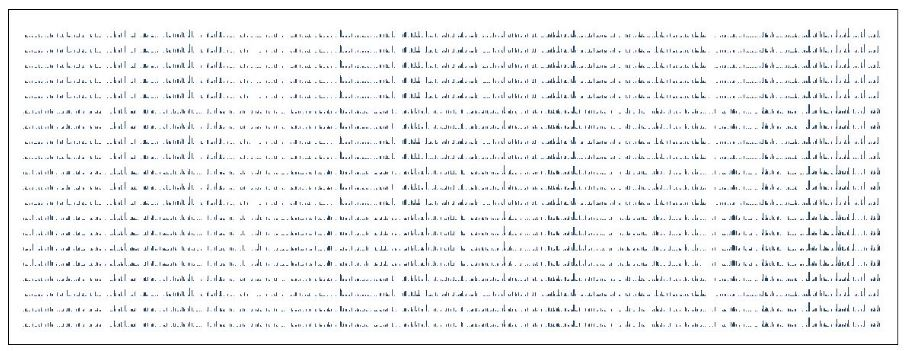
\includegraphics[width=\textwidth]{figs/8/spark_diagram}
    \caption{A 20-feature spark diagram}
    \label{fig:spark_problem}
\end{figure}

\begin{figure}[H]
    \centering
    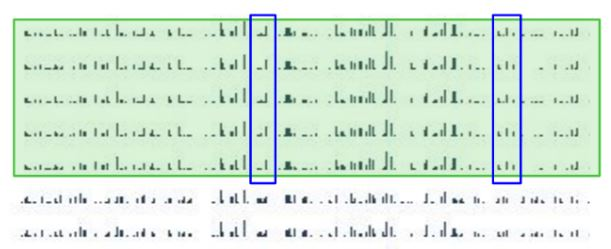
\includegraphics[width=\textwidth]{figs/8/spark_solution}
    \caption{ A subtle pattern that distinguishes vectors of Trees (highlighted in green) from the vectors of all other features}
    \label{fig:spark_solution}
\end{figure}

To achieve this, the classifier must be able to perform two key functions:
\begin{itemize}
    \item Learn - used to train the classifier via supervised learning
    \item Guess - used to receive the classifier's predictions regarding the class of an attribute vector
\end{itemize}

\section{Background Research}
There are a number of classification algorithms available, each with their strengths and limitations. For our problem, the classification algorithm must be capable of:
\begin{itemize}
    \item Handling high-dimensional input
    \item Learning quickly
    \item Learning iteratively
    \item Identifying a dynamic number of classes
\end{itemize}

\newpage
\subsection{Perceptron}
A binary perceptron provides a simple approach for determining if a given input belongs to a specific class or not. Given inputs 1 to N $x_n$, multiply each input by its corresponding weight 1 to N $w_n$, and if the sum of this reaches a threshold $T$, the input is predicted to belong to the class \citep{perceptron} (See figure \ref{fig:perceptron_img}).
$$ 
x \text{ belongs to class} = 
\begin{cases}
\mbox{True} &
\sum_{n=1}^{N} (x_n \cdot w_n) \geq T \\
\mbox{False} & \text{otherwise}
\end{cases}
$$

\begin{figure}[H]
    \centering
    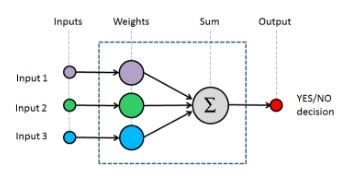
\includegraphics{figs/8/perceptron_img}
    \caption{Perceptron Structure}
    \label{fig:perceptron_img}
\end{figure}

Strengths:
\begin{itemize}
    \item Quick and easy to implement
\end{itemize}
Limitations:
\begin{itemize}
    \item Can only provide linear solutions
    \item Requires significant training data to make accurate predictions
    \item Ineffective with high-dimensional input
    \item Can’t solve the XOR problem
\end{itemize}
Time Complexity:
\begin{itemize}
    \item Learn: O(c) - but extensive training required
    \item Classify: O(c) - but poor accuracy unless sufficiently trained
\end{itemize}
\citep{perceptron_2}

\subsection{Neural Network}
A neural network consists of a number of perceptrons, arranged in layers such that the output from one perceptron feeds into the input of the next perceptron. The n-dimensional input is passed to m perceptrons in the input layer and fed through the neural network. Upon reaching the output layer, probabilities are provided for the input belonging to each class known by the network. If the prediction is incorrect, the process is reversed and the weightings of each node are modified accordingly \citep{neuralnetwork} (See diagram below \ref{fig:neuralnetwork_img}). 

\begin{figure}[H]
    \centering
    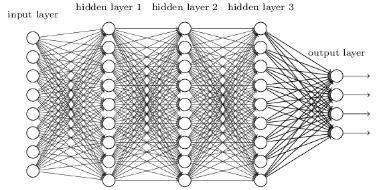
\includegraphics{figs/8/NN_img}
    \caption{Neural Network structure}
    \label{fig:neuralnetwork_img}
\end{figure}

Strengths:
\begin{itemize}
    \item Can provide linear and nonlinear solutions
    \item Requires less training than the perceptron
    \item Can achieve high levels of accuracy
    \item Provides probability estimates
\end{itemize}

Limitations:
\begin{itemize}
    \item Still requires a large amount of training data
    \item Ineffective with high-dimensional input
    \item Has a complex design that requires significant fine-tuning
    \item Can only classify a static number of classes
\end{itemize}

Time Complexity:
\begin{itemize}
    \item Learn: O($N^{L}$) - where N is the number of input nodes and L is the number of layers
    \item Classify: O($N^{L}$) - where N is the number of input nodes and L is the number of layers
\end{itemize}

\subsection{Support Vector Machine (SVM)}
An SVM maps n-dimensional input into an n-dimensional space, and find planes that separate each class while maximising the distance between them. Then, given some n-dimensional input, it predicts the class of the input based on which side of the separating plane it falls on \citep{svm} (see figure \ref{fig:svm_img}) 

\begin{figure}[H]
    \centering
    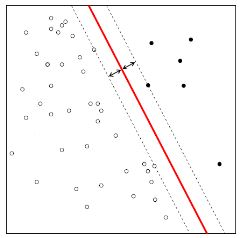
\includegraphics{figs/8/linear_svm}
    \caption{Diagram of SVM showing plane separating two classes}
    \label{fig:svm_img}
\end{figure}

Strengths:
\begin{itemize}
    \item Can provide linear and nonlinear solutions
    \item Effective with high-dimensional input
    \item Requires significantly less training than Neural Networks or Perceptrons
    \item Supports iterative learning
\end{itemize}

Limitations:
\begin{itemize}
    \item Unable to directly provide probability estimates
    \item Performs poorly as the number of classes increases
\end{itemize}

Time Complexity:
\begin{itemize}
    \item Learn: O(N) - where N is number of data entries
    \item Classify: O(n) - where n is the number of classes
\end{itemize}

\section{Design}
\subsection{Design Decisions}
\subsubsection{Classification Algorithm}
The SVM was selected since it best suited the needs of the project:
\begin{itemize}
    \item It requires little training data, which improves the system’s usability
    \item It handles high-dimensional input effectively, which is essential since the input has 1024 dimensions
    \item It supports iterative learning across a dynamic number of classes, which are strict requirements of the system
\end{itemize}

A number of machine learning libraries are available in python, but scikit-learn was selected as it provides a range of well implemented and well documented classification algorithms for free \citep{scikit-learn}.

One drawback of the SVM is that it can’t directly probability estimates. While these can be calculated based on the distance of a point to its surrounding separating planes, these values proved to be inaccurate, often contradicting the actual prediction of the SVM.  However, the implementation of Olivia allows probabilities to be obtained using contextual classification. By default, the attributes extracted by Olivia are based on the centre pixel of a 256x256 image, using the surrounding 192x192 pixels as context, and ignoring the outer 32 pixels on each side.

\begin{figure}[H]
    \centering
    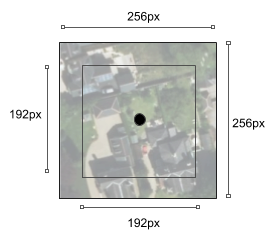
\includegraphics{figs/7/tile_range}
    \caption{Default image extraction zone}
\end{figure}

Contextual classification is the process of shifting Olivia’s focus point to 9 different positions in the image, such that every pixel is \textit{included as context}. This achieves 9 unique classifications per image, allowing probability estimates to be calculated from the results of these classifications.

\subsubsection{Linear SVM vs Non-Linear SVM}
There are a number of varieties of SVM, including linear and nonlinear SVMs. Linear SVMs separate classes with a linear plane (\ref{fig:linear_svm}), while non-linear SVMs use a Kernel function to transform each point and map them into a new space, in which a linear separation plane is found. The transformation makes it equivalent to using a curved line in the original input space, enabling higher accuracy and providing a solution to problems that can’t be solved with a Linear SVM. (\ref{fig:non_linear_svm}). 
\begin{figure}[H]
    \centering
    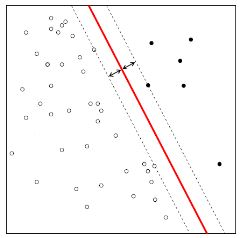
\includegraphics{figs/8/linear_svm}
    \caption{Linear SVM}
    \label{fig:linear_svm}
\end{figure}

\begin{figure}[H]
    \centering
    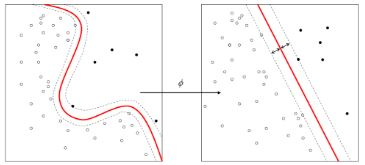
\includegraphics{figs/8/non_linear_SVM}
    \caption{Non-Linear SVM}
    \label{fig:non_linear_svm}
\end{figure}

By developing a test that mimics the use of the classifier within the system, the performances of both flavours was compared, allowing for the optimal approach to be selected. The following test was devised:
\begin{itemize}
\item 4 feature classes
\item 5 entries per class (20 data entries in total)
\item 4 entries per class given as training data.
\item Asked to predict the final entry
\item Entries rotated round-robin-style for a total of 20 tests
\item Overall accuracy calculated by percentage of correct predictions
\end{itemize}
In this test, the linear SVM had an top-1 accuracy of 80\%, while the non-linear SVM’s accuracy was only 65\%. This is likely due to the large-dimensional input, which increases the chances of a linear separating plane existing, allowing the linear SVM to perform well, while significantly more fine-tuning and training data would be required for an accurate nonlinear plane to be formed. Therefore, a linear SVM was selected.

\subsubsection{1vAll vs 1v1}
Another variety of SVM to consider is 1vAll or 1v1. The 1vAll SVM separates each class from all other classes using a single separating plane (\ref{fig:1vAll}, producing N SVMs, whereas a 1v1 SVM separates each class from each other class, resulting in $\frac{N(N-1)}{2}$ planes where N is the number of classes (\ref{fig:1v1}). 
\begin{figure}[H]
    \centering
    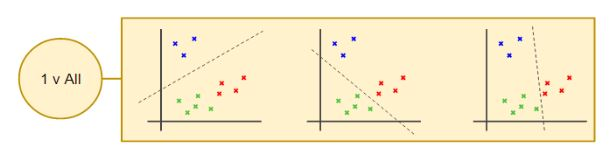
\includegraphics{figs/8/1vall_svm}
    \caption{1 vs All SVM - separating planes}
    \label{fig:1vAll}
\end{figure}
\begin{figure}
    \centering
    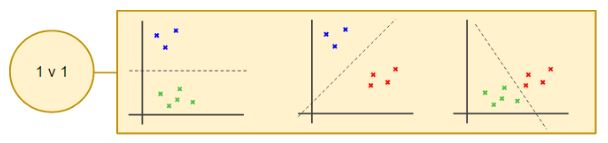
\includegraphics{figs/8/1v1_svm}
    \caption{1 vs 1 SVM - separating planes}
    \label{fig:1v1}
\end{figure}

Following the same test as above, 1v1 achieved top-1 80\% accuracy whereas 1vAll only achieved 55\% accuracy. 
However, 1v1 scales poorly as the number of classes increases, requiring (n-1)! separating planes to be calculated, compared to 1vAll which only requires n.
Overall the accuracy of the system was prioritised over its speed, so the 1v1 approach was selected.

\subsubsection{ Iterative learning: Partial Fit vs Knowledge Persistence}
A concrete requirement for the system is its ability to learn iteratively, allowing users to provide training data in increments rather than one large batch.

SVM has a ``partial fit” function, whereby the separating planes can be incrementally modified as the SVM’s knowledge increases. However, since the user would likely train the classifier one class at a time, providing batches of data belonging to that class, this was shown to cause the SVM to overfit for the class it was most recently trained with, significantly impacting its accuracy.

An alternative solution was to store all of the training data passed to the SVM. As new training data is provided, it can combine this with all previous data, and perform a regular fit. This not only eliminates the problem of overfitting, but also allows control over the SVMs knowledge, such that information can be un-learned by removing the entry from memory.
The cost to this approach is a memory requirement of the system that increases with the SVMs training. However, if this becomes an issue a remote database could be used instead.
Therefore, the knowledge persistence approach was selected.

\section{Implementation}
\subsection{Class Lookup Table}
The class lookup table provides an auxiliary function for converting human-readable feature names to SVM-useable ID numbers. This is achieved by a lookup table that maps feature_name to class_id. The table is implemented as a CSV file, and the user can dynamically add/remove entries to/from this table via the user interface. A unique class ID number is generated whenever the user adds a new class. If the user removes a class, training data belonging to that file is also removed from the SVM’s memory. 

\subsection{Classifier Knowledge Persistence}
The SVM’s knowledge persistence is again implemented using a CSV file. 
On start-up, it reads all previous training data from the CSV file into two arrays: attribute\_vectors and class\_ids. If it contains no previous training data, it uses the default training data file, containing data for 4 default classes: tree, road, building and house. If this file doesn’t exist, the arrays are left empty.
As additional training data is provided, it is appended to the two arrays. On shutdown, all data in the arrays is written back to the CSV in the format: [class\_id, attribute\_vector].

\subsection{Learn Function}
The learn function, along with the guess function, make up the core functionality of the classifier. The learn function’s implementation is as follows:
\begin{itemize}
    \item On start-up, reads all data from storage into the attribute\_vectors and class\_ids arrays
    \item Accepts a dictionary of [image url : attribute vector] and an array of corresponding feature names 
    \item Uses the Class Lookup Table to convert the feature name to its class ID
    \item Appends the new attribute vectors to the attribute\_vectors array, and the new class IDs to the class\_ids array
    \item If the data in the arrays only corresponds to a single class, returns a message informing the user that data for at least two classes is required before the SVM can fit 
    \item Else, performs a fit using all data provided and returns a success message
\end{itemize}

\subsection{Guess Function}
The guess function is implemented as follows:
\begin{itemize}
    \item On start-up, reads all data from storage into the attribute_vectors and class_ids arrays
    \item Accepts a dictionary of [image url : attribute vector]
    \item If the SVM hasn’t yet received sufficient data to perform a fit, returns an error message informing the user that further training across additional classes is required
    \item Else, predicts the class ID of each attribute vector
    \item Uses the Class Lookup Table to convert the class ID to a human-readable feature name
    \item Returns a dictionary of [image url : predicted feature name]
\end{itemize}

\section{Testing}
\subsection{SVM Testing}
Regression testing was used to ensure the guessing accuracy of the SVM didn’t deviate when trained on the same sets of data. This ensures that the library used performs consistently with our training data while learning iteratively using several refits.

Unit testing was used to test the knowledge persistence of the SVM. Firstly, the test verified that the SVM used previous data from the CSV file on startup. Secondly, it tested that, if this file doesn’t exist, the default training data is used. Finally it tested that, new training data is provided via the learn function, this data is correctly written to the CSV file, even when the SVM is shut down unexpectedly.
\subsubsection{Class Lookup Table Testing}
Unit testing was used to check all aspects of the Class Lookup Table’s functionality.

Firstly, it was ensured that classes could be added or removed from the table correctly. Additionally, upon removing a class, the test ensured that all corresponding data entries were removed from the SVM’s memory. 

Secondly, the functions for finding a class ID from its name and vice versa were tested. The test ensured these functions behaved consistently as new classes were added and removed.
\subsubsection{Endpoint Testing}
The endpoints of the classifier microservice were tested to ensure they behaved correctly with valid input, and returned an appropriate error message when given invalid input.

Unit tests were developed to ensure the Learn Endpoint responded correctly to the following cases:
\paragraph{Valid Input\\}
\tab Returns Success
\paragraph{Invalid Input: the number of vectors doesn’t match the number of class IDs\\}
\tab Returns Length Mismatch Exception
\paragraph{Edge case: the classifier has only been given training data for a single class\\}
\tab Returns Not Ready To Predict Message

Similar tests were developed for the Guess Endpoint:
\paragraph{Valid Input\\}
\tab Returns Success
\paragraph{Invalid input: list of vectors is empty\\}
\tab Returns Empty List Exception
\paragraph{Edge case: the classifier has only been given training data for a single class\\}
\tab Returns Not Ready To Predict Message

\section{Limitations}
The design decisions and implementation of the classifier result in the following limitations:

Firstly, the SVM algorithm scales poorly as the number of classes increases, especially when using the 1v1 variety, as significantly more separating planes must be computed. Additionally, further training data is often required in this case as the space between classes typically  reduces. However, this effect is reduced due to the high-dimensional data used by the system. 

Secondly, storing all training data in a CSV file adds an additional memory requirement to the system. Each data entry, consisting of a class ID and 1024 attribute values, is approximately 5kb in size. Alone this doesn’t pose as a significant problem, but since there is no confirmed upper boundary for the quantity of training data that would be used, there is the possibility of this becoming a significant overhead. If this becomes the case, the data would need to be moved to a remote database.

Finally, by fitting the SVMs separating planes using all learnt data while using a 1v1 variety, this could significantly increase the time taken to fit the graph. However, upon testing the time taken for a 1v1 SVM to fit its separating planes based on 10,000 data entries, this only took approximately 5 seconds, so is unlikely to be a problem.

\section{Evaluation}
Overall, the design and implementation of this classifier has ensured the key requirements of the system are met. 
The SVM algorithm is capable of efficiently handling high-dimensional data, requires minimal training from the user, and provides accurate predictions. Through the implementation of knowledge persistence, it is capable of learning iteratively, the number of classes can be modified dynamically and its knowledge can be easily managed.
One flaw of the SVM is its inability to directly give probabilities, but the use of contextual classification provided a workaround to this, albeit somewhat less precise.
However, while adaptations made to the classifier optimise its accuracy, functionality and utility, this comes at the cost of a design that scales poorly as the number of classes and training data increases.

\chapter{Saturn} \label{chapter:sat}
\section{Overview}
Saturn is the main co-ordinator service which acts as a bridge between the client facing service and the other backend services (i.e. Olivia and Classifier). It handles all the front-end HTTP requests and data that is being sent in either via x-www-form or JSON. Saturn has been through a number of evolutions due to the various stages of agile development. During initial development stage, Saturn was the only back-end service where every major computations were performed locally. At present, all complex computational operations are allocated to two remote services which are linked to Saturn. Below is the list of tasks that is handled by Saturn:

\begin{enumerate}
      \item Communicates with Olivia for extracting attributes from image tile
           \item  Communicates with Classifier to classify or reclassify the data
          \item Communicates with Classifier to get list of all data that belongs to certain theme
          \item   Communicates with Classifier to reset, delete and clear the data set
      \item Manages the `Discover’ sweep from the GUI
\end{enumerate}
\section{Design}
During the first iteration, the whole back-end system design was a single modular system based on Monolithic architecture. All the feature extraction and classification tasks were handled internally, by the single saturn server. Later, the design architecture was changed to micro-services where each major task is now allocated to remote services for computing. 

Saturn has dedicated modules for each server with specialised methods defined within it, to carry out certain functionality. For instance, it has an Olivia module which has a method called ``get\_all\_attr\_vecs(image\_list)” which takes a list of image URLs as parameter. When the method is invoked, it will then send the list to Olivia server for extracting the image’s attributes and returns a dictionary of URL as key with its corresponding attributes as values.
\begin{figure}[H]
    \centering
    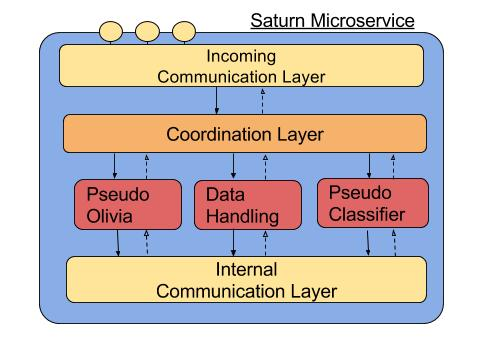
\includegraphics{figs/9/scl}
    \caption{Saturn Internal Communication Architecture}
    \label{fig:sat:scl}
\end{figure}
Figure \ref{fig:sat:scl} shows the internal structure of Saturn server where incoming request are handled by Incoming communication layer and transferred to Coordination layer. Coordination layer is linked to Olivia and Classifier module which are responsible for communicating with remote servers. Internal Communication layer handles all the data that is being communicated services `internal’ to the back-end.
\subsection{Data Handling}
As the main interface to the back end services, Saturn must have more complex data manipulation to handle a range of error inputs. It can accept x-wwww-form and JSON formatted data. When the server gets the request from front-end GUI, it will extract relevant provided data and repurpose it for use with the next services; removing any redundant or unnecessary pieces of data. This data is then converted to JSON to send to the next service. Having a structured style helps to maintain uniformity throughout the application system and avoids any kind of confusion during communication.

Saturn server has a list of endpoints that respond to certain tasks such as: finding them; classifying data; extracting attributes; clearing data; resetting data and downloading data. Certain endpoints merely act as routers, passing the message on. For example the saturn/clear endpoint triggers olivia/clear and classifier/clear. 
The key function within Saturn is the Feature Finder, or the `discover’ sweep from the GUI perspective. This service extensively uses the other services to perform its own computation to determine the class of each individual image tiles based on the returned data from Classifier. It has method that determines the class of the specific tiles based on its probability value. As mentioned earlier, each tile is computed nine times using the NSEW technique in Olivia (defined in section \ref{section:nsew}) and classified in Classifier. Using that returned data, Saturn assigns probability value to each tile requested based on their given feature type. Saturn will choose the class which has the highest probability value from among all nine tiles to determine class of single image tile.

\subsection{Error Handling}
Saturn ensures a uniformity in its returns by catching all the exceptions. Connection errors and connection timeout exceptions are two of the more frequently observed errors due to the issue . It also handles all the error message that is being passed from remote servers. It analyses the returned data and in case of any error found, it will include appropriate error messages to be transmitted to the front end. For instance, if Olivia failed to download and extract some of the image tiles attributes, it will first check if there is any failed image that is being returned. If yes then it will include the error message and returns the data to the front-end server in JSON format. This makes it much easier for client applications to consume saturn's data and encouraging them to communicate with saturn, ensuring the correct flow of service usage.

\subsection{Global Persistence vs Local Persistence}
Initial system design was to implement a global persistence system which acts as a main body for storing and communicating the data. However, this system design made other servers depended on Saturn as they will have to request for data every time to perform any task. This proved to be an ineffective way to program an application using micro-service architecture. Now Saturn doesn’t hold any data by itself. Each remote server store their data locally which Saturn can access by making data request. The reason for such design change was to make each service or server self-sufficient to perform the given task.
\section{Evaluation}
Saturn has a good communication architecture that can handle all the request from front-end GUI. It follows a structured messaging style to communicate the data which prevents any occurrence of human error when passing the data. Having a dedicated endpoint for each task makes it easier for front-end server to invoke the right endpoint. By tidying data and offering the feature finder as a macro function encourages clients to use Saturn rather than incorrectly using the other micro services. Overall Saturn performance is very good when it comes to coordinating task and communicating between the remote servers.

\include{chapters/10_results/results}
\chapter{Critical Evaluation} \label{chapter:Critical Evaluation}

\section{Time Management}
Overall, time management within the project was handled well. By using agile methodology throughout the project we constantly set new deadlines and targets to reach for the next sprint, and this helped ensure progress was consistently made from start to finish. This became more challenging in certain stages of the project due to coursework deadlines affecting how much work each team member was able to do, and as everyone took a different set of modules this meant that we had to constantly adjust to the availability of each other. With frequent scrums, the team was able to discuss availability and inform the rest of the group of any major deadlines, and this gave us the ability to alter workload to compensate around this. Another ethos that was used in the project which assisted situations such as these was our ‘minimum viable product’ ethos. As explained in our planning section, by ensuring there was always a minimum viable product, it meant that our tool was always fully functioning. The effect of this was that no task was mandatory to complete in order to make our product ‘work’, only to expand on it’s functionality, meaning that a majority of our features could be worked upon independently of one another without breaking someone else’s work.

There were times in our project where certain tasks took longer to complete than initially planned for. With other tasks depending upon the completion of these tasks, this had a knock-on effect, resulting in delays in progression. An example of this would be situations where the endpoints within the back-end of our application would be modified, and the user interface could not be updated until it was known exactly what form the back-end would now accept and return data in. Fortunately, each team member had enough tasks assigned so that the majority of the time, if someone was unable to work on one certain task, they could instead switch their focus to a different task. This was made much easier through the use of a project Trello board, so we knew what tasks were required to be done and could identify a different task to work on with ease.

In the early stages of our project, a Gantt chart, as can be seen in figure \ref{fig:gantt}, was created based off of our initial project goals and requirements, containing all major progress seminars and other deadlines. Agile development meant that during sprint planning meetings the team could assess which sections of the project were to be worked on during the next sprint, and could also identify a number of tasks based off of our Gantt chart that could be completed during the next sprint in order to reach progress targets. During deliverable one, we stuck to our Gantt chart almost perfectly, reaching all targets that had been aimed for. However, during this deliverable, in scrum meetings we started to identify that Terrapattern was not going to be the ideal solution for some of the project’s requirements, meaning that the direction of our project began to diverge from the Gantt chart. With agile, this was not a problem as the Gantt chart was simply an initial outline for main plans, and with sprints occurring every two weeks we were able to set targets with the project client on a per-sprint basis, whilst still ultimately working towards the main goals in the project.

\section{Requirements Analysis}
In order to evaluate the final product effectively, this section will refer back to requirements stated in the planning section, and document whether/how each requirement has been met.

\subsection{Functional Requirements}

This section addresses functional requirements as listed in \ref{funcreqs}.

\subsubsection{Image uploading}
The user is able to upload any Ordnance Survey image of any quality. Currently, upload is restricted to 4000x4000px due to lack of server resources making it infeasible to increase this limit, however the majority of images provided are 4000x4000px.

\subsubsection{Feature Selection}

A user is able to select any feature within the image. By using a grid of 128x128px and a selection size of 256x256px, features that lay on borders are able to be selected.

\subsubsection{Attribute Extraction}

The system successfully extracts information from selected features. It can extract 1024 attributes from any given image tile of size 256x256px. 

\subsubsection{Feature Identification}

The system successfully uses the extracted information to classify the selected feature using the SVM.

\subsubsection{Iterative Training}

``Learn Mode" in Productizer fully supports iterative training.

\subsubsection{Intuitive Interface}
The user interface is simple to use, and abstracts away from the complexity of the application.

\subsection{Non-Functional Requirements}

This section addresses our non-functional requirements as listed in \ref{nonfuncreqs}.

\subsubsection{Accuracy}
We were unable to fully test our accuracy beyond a limited set of sample imagery, however the application showed a high accuracy rate within all sample imagery with sufficient training.

\subsubsection{Scalability}
With use of an SVM, 100 features does have an effect on overall performance, however still provides the ability to classify this number of unique features.

\subsubsection{Speed}
The back-end meets our 0.1s target for image processing.

\subsubsection{Usability}
The user is typically required to provide 5 to 10 training images per feature to obtain accurate predictions. This can easily be achieved within 5 minutes via the user interface.

\subsubsection{Productivity}
We are unable to test this productivity requirement within the time frame of our project.

\subsection{Implementation Requirements}

This section addresses our implementation requirements as listed in \ref{impreqs}.

\subsubsection{Language}
The front and back end met the language requirements that we stated.

\subsubsection{Persistence}
The front and back end met all of our stated persistence requirements.

\subsubsection{Front End}
The front-end successfully can be accessed by multiple users concurrently.

\subsubsection{Platform}
The back-end operates on a platform that is available to a wide audience.

\subsubsection{Framework}
Flask proved to be quick to learn within the project timeframe, allowing it to be powerfully utilised within the final product.

\subsection{Interface Requirements}
This section addresses interface requirements as listed in \ref{intreqs}.

\subsubsection{Image Manipulation}
The interface of the application successfully allows a user to upload any Ordnance Survey aerial image and by using Google Maps API allows said user to pan around, selecting features as they desire. A history page on our web interface provides access to all previously uploaded images.

\subsubsection{Interaction with Classifier}
The user interface submits requests to the back-end based on data provided by the user, and provides data in a fashion that hides the complexity of all back-end algorithms. The interface is easy to use and requires no knowledge in machine learning.

\subsection{Use Case Analysis}
All processes stated within the use case diagram, as shown in figure \ref{fig:use_case_diagram}, have been satisfied. A user is able to use previous maps or upload a new one, use Learn Mode to teach the classifier, use Discover Mode to obtain predictions based on training data provided, and filter these predictions based on the class they are looking to find. They are able to create new classes that are defined on the classifier with sufficient training data, and finally reclassify a map to find any features that may change in class due to further training data.

\chapter{Further Work} \label{chapter:further}
The whole project was intended to be a prototype to see if feature classification could be implemented using OS images, hence this covered basic functionality. Allowing many ways to improve the current system. In some sections there are mentions of further work that are specific to a particular module. Due to the modularity associated with Microservices and the structure of our code, a solid foundation is set to enable extensions and improvements. This chapter includes some of these potential system improvements and extensions




\section{Improvements}


\subsection{Example training usage}
One outcome from the usability testing at OS was that users were not entirely sure how to classify various tiles. Given that tiles covered more than one specific type of feature e.g. a tile containing a house that backed onto a forest; they were unsure how to handle mixed theme tiles.

They suggested that a demonstration to be included on the web-site. This could be simply a collection of images and what classifications they should be deemed as. This would provide a guide and more confidence to the users when the Productizer is in learn mode. This could be included in the learn mode, scrolling down to see it. 




\subsection{Required Training Indicator}
One issue we observed through the usability testing was that the users assumed the system was ready to `discover' features far earlier than it would be recommended to. This resulted in bad or obviously untrustworthy classifications from the `discover sweep'. To account for this there should be stricter control over when user trains classifier on any given theme. This can be achieved by implementing some kind of GUI based indicator bar within the site that will hint the user on how many more tiles for each feature type are required to ensure a respectable and reliable outcome. 


\subsection{Normal Curve Context}
The current implementation extracts `context' from inside the tile and only the tile. As a result there is an issue when classifying regions that are bigger than a tile. For example the difference between a pond and lake or a larger private garden or public park. Features are normally very related to their surroundings. The NSEW approach ignores  surrounding tiles.

A way to solve this would be by extending the context to a larger number of tiles. The solution would involve two stages of classification in order to determine the final classification: 
\begin{enumerate}
\item Classification of all the NSEW generated sub-tiles
\item A weighted sum of classifications where the weighting is determined by a bell curve

\end{enumerate}

The first classification is the same as the current format however the resulting label of each sub-tile would be stored in graph of nodes. This would created a 2D network, where every node has an x and y position and a class label. 


The second classification would look at each tile $t$ and weigh each surrounding node based on its position on the bell curve. The bell curve would have a mean $ \mu $ (or centre) of the centre of the tile $\mu = \begin{bmatrix}x_t \\ y_t \end{bmatrix}.$

\begin{figure}[H]
    \centering
    \includegraphics[width=\textwidth]{figs/12/3d_normal}
    \caption{A 3D representation of the normal curve}
    \label{fig:fw:3d_normal}
\end{figure}

Previously a tile would contain 9 nodes (each NSEW result) and each classified node would carry a weight of $11.1\%$. 
In the proposed method, nodes outside the tile will have an influence on the final classification. 
Figure \ref{fig:fw:3d_normal} shows that weight. 
The distance of a node $n = \begin{bmatrix}x_n \\ y_n \end{bmatrix}$
from the centre of the tile provides an weight of $P(T = n)$ 
such that $T \sim \mathcal{N}(\mu,\,C)\,$, 
where the co-variance $C  =\begin{bmatrix}\sigma^2 & 1 \\ 1 & \sigma^2 \end{bmatrix}$.\\
Minor normalisation might have to occur, in order to prevent a total of 100\%. 
Therefore probability for a tile $t$ belonging to any class $f$:

$$ 
P(f | t)  =
\Phi \Bigg(
\sum_{i=(x_t-2\sigma)}^{(x_t+2\sigma)}
\sum_{j=(y_t-2\sigma)}^{(y_t+2\sigma)}
\Big(
\lambda_{i,j}(f) \cdot P(T = t)
\Big)
\Bigg)
$$

Such that $\Phi(x)$ is the normalisation function and the binary function $\lambda_{i,j}(f)$ equals 1 if the node at [i,j] was initially classified as feature $f$ and 0 otherwise.


$$
\lambda_{i,j}(f) = 
\begin{cases}
\mbox{1} & \text{if SVM.classify}(n) = f\\
\mbox{0} & \text{otherwise}
\end{cases}
$$

The winning feature $\hat{f}$ for the tile would be the feature with the highest probability:
$P(\hat{f}|t) > P(f|t)\ \forall f \neq \hat{f}$. 






\subsection{Required Training Indicator}
Given an incorrect classification, currently a user must switch from discover to learn mode; then find the incorrectly labelled tile and correctly retrain the model with that feature. This raises two issues. Switching from discover to learn mode removes all the markers. Which firstly, makes it difficult to find the exact tile. Secondly you cannot see what it was classified as. 

To solve this, there should be some sort of button allowing the user to make an amendment on the discover mode. Based on the design of the system, it would be (computationally) optimal for the user to queue a number of corrections. As batches of information take less time to process. However this may be less intuitive. To counter this, the queue should be hidden from the user. The classification will enter a pending state, where it will await for the user to change mode or click the reclassify button. Changing mode would send all amendments to Saturn as if it was a standard learn mode with mixed label data. If the user clicked `reclassify' originally, a discover sweep would occur. However in this case a hidden (i.e. the user will not be informed) learn command (without changing to learn mode) would be sent, followed by a `discover' sweep, so that the changes affect the reclassification.  





\section{Extensions}
\subsection{Automation of learning via MasterMap}
OS has a number of map products containing all sorts of information. Their flagship product is `OS MasterMap'. It contains over 470 million features and is constantly being updated (10,000 features a day, \cite{OS:Youtube}). The classifications of these features is expansive, such as marshes, post offices, pylons, telephone boxes and more. This expansive amount of labelled data could be used to replace the human operator during training. MasterMap also has a aerial imagery layer. As the two products are MasterMap, their coordinate system would match, therefore creating corresponding tiles would be trivial. By automating the process of learning the data, an operator needs only to correct mistakes. Which would mainly be edges cases.

Once a selection of tiles has been generated, the issue of classifying a tile arises. This could  be solved in two ways. The first way could be by determining how much of the tile is covered by each feature within a tile area and the tile is classified as the feature with the largest area. The second method would mimic the NSEW approach. Where nine points are taken from the tile in the same location as the nine focus points of the NSEW approach. The feature type at that exact location would be a vote for that feature type. The feature type with the most vote claims the tile.

\begin{figure}[H]
    \begin{minipage}{0.5\textwidth}
  \centering
  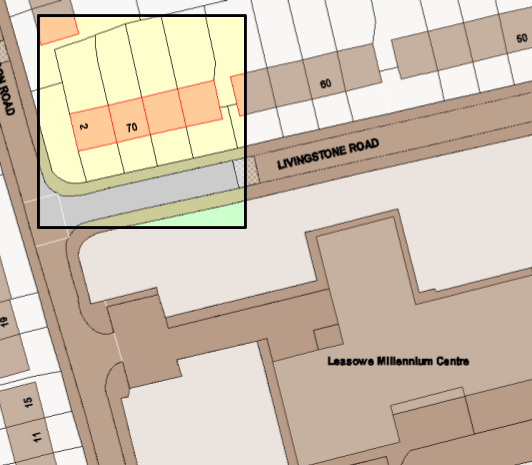
\includegraphics[width=0.95\textwidth]{figs/12/osmm_m1}
  \caption{Method 1}
  \label{fig:sub2}
\end{minipage}\hfill
\begin{minipage}{0.5\textwidth}
  \centering
  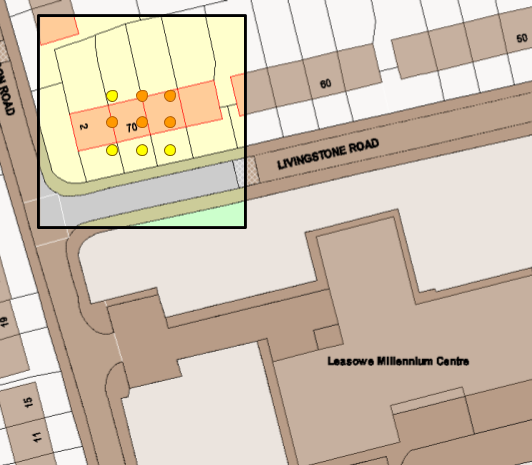
\includegraphics[width=0.95\textwidth]{figs/12/osmm_m2}
  \caption{Method 2}
  \label{fig:sub2}
\end{minipage}
\caption{Two methods of choose a class for a tile}
\label{fig:FW:methods}

\end{figure}



If we compare the two methods in the example in Figure \ref{fig:FW:methods}, the second method seems more optimal. Housing wins with a vote of 5 to 4 for gardens, whereas the first method would result in garden as it obviously has the largest area (yellow). However this would need to be experimented as this is a single case; a potentially more complex method might need to be adopted. 

No internal code changes are required, due to the nature of the micro-services. However, a new simple controller would be needed, to orchestrate the task. Assuming the tagging of tiles before training the model can be achieved, this allows for more training data to be processed in less time. The more a model is trained, the more reliably it can classify the correct feature to a tile. This allows the model to rapidly update when a new collection of data arrives. By training it on random tiles it can quickly learn the entire new dataset and propagate the knowledge classifying all of it.







\subsection{Discover Feature Outlines}
A common theme that resonates throughout the system is the issue with tiles. Raw tiling is a flawed system for identifying specific features. Within a single tile there could be multiple features that we have to generalise to a single feature; resulting in an effective loss of data. 

If we could extract objects from a tile, we could then attempt to classify the single objects. This can be done by in a number of ways. A simple yet effective method would be edge detection, the most appropriate method from similar works seems to be the Sobel method with a binary gradient mask in order to determine object outlines \citep{sobel_method}. The outlines can then be applied to cut the objects from the tile. 

\begin{figure}[H]
    \centering
    \includegraphics[width=\textwidth]{figs/12/sobel}
    \caption{Potential results of object extraction}
    \label{fig:FW:sobel}
\end{figure}

Figure \ref{fig:FW:sobel} shows an example of what you would hope the edge detection would produce. Note that a light green colour was taken to show that the remaining image has been ignored. With these new images each region \textbf{within} a tile can be classified, also leaving unknown or miscellaneous regions that request human assistance. More importantly this would produce a more precisely classified map. As can be shown in the figure \ref{fig:FW:object_class}, the results are quite dramatically different. 

\begin{figure}[H]
    \centering
    \includegraphics[width=\textwidth]{figs/12/new_classes}
    \caption{Comparison of Object classification verses tiling classification}
    \label{fig:FW:object_class}
\end{figure}
\chapter{Conclusion} 
\label{chapter:conclusion}
The aim of this project was to build an easy-to-use web application that allows Ordnance Survey employees to upload a complex aerial photograph, and train the system to identify and label specific features on this image and other similar images. Employees can train the system with supervised learning data by selecting features on the uploaded image and providing labels for these features. At the click of a button, the system can then propagate this knowledge across any given map image to label other occurrences of these features. Employees can dynamically add new classes to the system, and iteratively provide additional training data to be added to the system’s knowledge-base, enhancing its ability to identify new and existing features. The vast complexity that operates behind the scenes is abstracted from the user, meaning that no previous knowledge in machine learning is required to operate the system. 

These functional requirements of the application were not only achieved, but also optimised to improve the performance of the system while providing an intuitive and enjoyable user experience. Additionally, the project was implemented with a modular and expandable code base, allowing for the prototype to be modified, improved and extended as required by the customer. 

By working under an agile methodology any obstacles that arose during the project could be efficiently tackled, and changes to the initial project goals could be catered for, ultimately creating a stronger, more effective and conclusively successful final product. As a prototype application, the project opens itself up to a wide range of future extensions and improvements that will only enhance the already powerful tool that has been created.



\appendix
\chapter{Project Proposal} \label{appendix_proposal}
\include{appendix/proj_reqs}


\backmatter
\bibliographystyle{ecs}
\bibliography{ECS}
\end{document}
%% ----------------------------------------------------------------
